%% ----------------------------------------------------------------
%% Thesis.tex -- MAIN FILE (the one that you compile with LaTeX)
%% ---------------------------------------------------------------- 

% Set up the document
\documentclass[a4paper, 11pt, twoside]{Thesis}  % Use the "Thesis" style, based on the ECS Thesis style by Steve Gunn
\usepackage[spanish]{babel}
\selectlanguage{spanish}
\usepackage[utf8]{inputenc}

%\usepackage{draftwatermark}
%\SetWatermarkText{DRAFT}
%\SetWatermarkScale{5}

\graphicspath{{Figures/}}  % Location of the graphics files (set up for graphics to be in PDF format)

\usepackage[utf8]{inputenc}
% Include any extra LaTeX packages required
\usepackage[square, numbers, comma, sort&compress]{natbib}  % Use the "Natbib" style for the references in the Bibliography
\usepackage{verbatim}  % Needed for the "comment" environment to make LaTeX comments
\usepackage{vector}  % Allows "\bvec{}" and "\buvec{}" for "blackboard" style bold vectors in maths
\hypersetup{urlcolor=blue, colorlinks=true}  % Colours hyperlinks in blue, but this can be distracting if there are many links.

\usepackage{fancyvrb}
\fvset{frame=lines,numbers=left,numbersep=3pt}

\usepackage{emp}
\empprelude{input graph}
\DeclareGraphicsRule{*}{mps}{*}{}

\usepackage{tikz}
\usetikzlibrary{arrows,shadows} % for pgf-umlsd

\usepackage[underline=true,rounded corners=false]{pgf-umlsd}
%Utilización de sensores para controlar aplicaciones web desarrolladas con continuations
%Adaptabilidad al contexto en aplicaciones web desarrolladas con continuations
\newcommand{\thesisTitle}{Adaptabilidad al contexto en aplicaciones web desarrolladas con continuations}
\newcommand{\thesisMailTitle}{Adaptabilidad al contexto en aplicaciones web desarrolladas con continuations}
\newcommand{\thesisAuthor}{Eloy Adonis Colell}

\setcounter{secnumdepth}{2}
\setcounter{tocdepth}{2}

%% ----------------------------------------------------------------
\begin{document}
\begin{empfile}[Thesis.uml]
\begin{empcmds}
input metauml;
\end{empcmds}

\frontmatter	  % Begin Roman style (i, ii, iii, iv...) page numbering

% Set up the Title Page
\title  {\thesisTitle
			%\\
			%{ \Large ¿Cómo utilizar los sensores del cliente?}
			}
\authors  {\texorpdfstring
            {\href{mailto:eloy.colell@gmail.com?subject=\thesisMailTitle}{\thesisAuthor}}
            {\thesisAuthor}
            }
\addresses  {\groupname\\\deptname\\\univname}  % Do not change this here, instead these must be set in the "Thesis.cls" file, please look through it instead
\def\today{\ifcase\month\or
  Enero\or Febrero\or Marzo\or Abril\or Mayo\or Junio\or
  Julio\or Agosto\or Septiembre\or Octubre\or Noviembre\or Diciembre\fi
  \space \number\year}
\date       {\today}
\subject    {}
\keywords   {}

\maketitle
%% ----------------------------------------------------------------

\setstretch{1.3}  % It is better to have smaller font and larger line spacing than the other way round

% Define the page headers using the FancyHdr package and set up for one-sided printing
\fancyhead{}  % Clears all page headers and footers
\rhead{\thepage}  % Sets the right side header to show the page number
\lhead{}  % Clears the left side page header

\pagestyle{fancy}  % Finally, use the "fancy" page style to implement the FancyHdr headers

%% ----------------------------------------------------------------
% Declaration Page required for the Thesis, your institution may give you a different text to place here
\Declaration{

\addtocontents{toc}{\vspace{1em}}  % Add a gap in the Contents, for aesthetics

Yo, \thesisAuthor, declaro que este documento titulado, `\thesisTitle' y el trabajo presentado son de mi propiedad. Y confirmo que:

\begin{itemize} 
\item[\tiny{$\blacksquare$}] Este trabajo fue totalmente hecho mientras realizaba la candidatura para la investigación de grado en esta Universidad.
 
\item[\tiny{$\blacksquare$}] Cuando una parte de esta tesis ha sido previamente enviada para una evaluación de nivel o alguna otra calificación a esta Universidad u otra institución, esto ha sido claramente fijado.
 
\item[\tiny{$\blacksquare$}] Cuando he consultado el trabajo publicado de otros, esto ha sido mencionado.
 
\item[\tiny{$\blacksquare$}] Donde he citado el trabajo de otro, la fuente siempre ha sido dada. Con la excepción de dichas citas, esta tesis es enteramente de mi propiedad.
 
\item[\tiny{$\blacksquare$}] He reconocido todas las fuentes principales de ayuda.
 
\item[\tiny{$\blacksquare$}] Cuando me basé en el trabajo hecho por mi mismo en conjunto con otros, he dejado exactamente claro que parte fue hecha por los otros y cual fue mi contribución a ese trabajo.
\\
\end{itemize}
 
 
Firma:\\
\rule[1em]{25em}{0.5pt}  % This prints a line for the signature
 
Fecha:\\
\rule[1em]{25em}{0.5pt}  % This prints a line to write the date
}
\clearpage  % Declaration ended, now start a new page

%% ----------------------------------------------------------------
% The "Funny Quote Page"
\pagestyle{empty}  % No headers or footers for the following pages

\null\vfill
% Now comes the "Funny Quote", written in italics
%\textit{``Success is the ability to go from failure to failure without losing your enthusiasm.''}\\
\textit{``Dar el ejemplo no es la principal manera de influir sobre los demás; es la única manera.''}

\begin{flushright}
Albert Schweitzer
\end{flushright}

\vfill\vfill\vfill\vfill\vfill\vfill\null
\clearpage  % Funny Quote page ended, start a new page
%% ----------------------------------------------------------------

% The Abstract Page
\addtotoc{Resumen}  % Add the "Abstract" page entry to the Contents
\abstract{
\addtocontents{toc}{\vspace{1em}}  % Add a gap in the Contents, for aesthetics
En este trabajo se crea una alternativa para utilizar los sensores provistos por un navegador web desde una aplicación web desarrollada con continuations.

Diseñar dicha alternativa, contempla mezclar 2 lineas de investigación que contienen requisitos contrapuestos: la sensibilidad al contexto y las aplicaciones web desarrolladas con continuations.

Por último se presenta un ejemplo, al cual se le agrega adaptación al contexto, y se evalúa la extensibilidad y los limites de la alternativa propuesta.

Finalmente se discute el trabajo en forma global, presentando las principales diferencias con las alternativas actuales.
}

\clearpage  % Abstract ended, start a new page
%% ----------------------------------------------------------------

\setstretch{1.3}  % Reset the line-spacing to 1.3 for body text (if it has changed)

% The Acknowledgements page, for thanking everyone
\acknowledgements{
\addtocontents{toc}{\vspace{1em}}  % Add a gap in the Contents, for aesthetics

Primero deseo agradecer a mi Director, el Mg. Javier Bazzocco por su guía y ayuda en el desarrollo de mi tesis.

También me gustaría agradecer a mi Co-Director, el Prof. Dr. Alejandro Fernández que me motivó a aprender Smalltalk y unirme al LIFIA.

Además me gustaría agradecer a Lucas Capalbo por sus lecturas cuidadosas y comentarios constructivos que me ayudaron al mejoramiento de esta tesis.

Por último me gustaría agradecer a mis padres, por todo el ánimo y apoyo durante mis estudios. 

}
\clearpage  % End of the Acknowledgements
%% ----------------------------------------------------------------

\pagestyle{fancy}  %The page style headers have been "empty" all this time, now use the "fancy" headers as defined before to bring them back


%% ----------------------------------------------------------------
\lhead{\emph{Índice general}}  % Set the left side page header to "Contents"
\tableofcontents  % Write out the Table of Contents

%% ----------------------------------------------------------------
\lhead{\emph{Índice de figuras}}  % Set the left side page header to "List if Figures"
\listoffigures  % Write out the List of Figures

%% ----------------------------------------------------------------
\lhead{\emph{Índice de cuadros}}  % Set the left side page header to "List of Tables"
\listoftables  % Write out the List of Tables

%% ----------------------------------------------------------------
\setstretch{1.5}  % Set the line spacing to 1.5, this makes the following tables easier to read
\clearpage  % Start a new page
\lhead{\emph{Abreviaciones}}  % Set the left side page header to "Abbreviations"
\listofsymbols{ll}  % Include a list of Abbreviations (a table of two columns)
{
%\textbf{AJAX} & \textbf{A}synchronous \textbf{J}avascript \textbf{A}nd \textbf{X}ML\\
\textbf{API} & \textbf{A}pplication \textbf{P}rogramming \textbf{I}nterface\\
\textbf{COP} & \textbf{C}ontext \textbf{O}riented \textbf{P}rogramming\\
\textbf{CPS} & \textbf{C}ontinuation-\textbf{p}assing \textbf{S}tyle\\
%\textbf{CSS} & \textbf{C}ascading \textbf{S}tyle \textbf{S}heets\\
%\textbf{GPS} & \textbf{G}lobal \textbf{P}ositioning \textbf{S}ystem\\
\textbf{HTML} & \textbf{H}yper\textbf{T}ext \textbf{M}arkup \textbf{L}anguage \\
\textbf{HTTP} & \textbf{H}yper\textbf{t}ext \textbf{T}ransfer \textbf{P}rotocol \\
%\textbf{JVM} & \textbf{J}ava \textbf{V}irtual \textbf{M}achine\\
\textbf{MVC} & \textbf{M}odel \textbf{V}iew \textbf{C}ontroller\\
%\textbf{OSC} & \textbf{O}ctopus \textbf{S}easide \textbf{C}ognizance\\
%\textbf{OS} & \textbf{O}perative \textbf{S}ystem\\
%\textbf{P2P} & \textbf{P}eer \textbf{(to)} \textbf{P}eer\\
\textbf{QoS} & \textbf{Q}uality \textbf{o}f \textbf{S}ervice\\
\textbf{REST} & \textbf{Re}presentational \textbf{S}tate \textbf{T}ransfer\\
\textbf{URL} & \textbf{U}niform \textbf{R}esource \textbf{L}ocator\\
\textbf{UML} & \textbf{U}nified \textbf{M}odeling \textbf{L}anguage\\
%\textbf{XML} & E\textbf{x}tensible \textbf{M}arkup \textbf{L}anguage\\
\textbf{WWW} & \textbf{W}orld \textbf{W}ide \textbf{W}eb\\
}

%% ----------------------------------------------------------------
%\clearpage  % Start a new page
%\lhead{\emph{Physical Constants}}  % Set the left side page header to "Physical Constants"
%\listofconstants{lrcl}  % Include a list of Physical Constants (a four column table)
%{
% Constant Name & Symbol & = & Constant Value (with units) \\
%Speed of Light & $c$ & $=$ & $2.997\ 924\ 58\times10^{8}\ \mbox{ms}^{-\mbox{s}}$ (exact)\\
%
%}

%% ----------------------------------------------------------------
%\clearpage  %Start a new page
%\lhead{\emph{Symbols}}  % Set the left side page header to "Symbols"
%\listofnomenclature{lll}  % Include a list of Symbols (a three column table)
%{
% symbol & name & unit \\
%$a$ & distance & m \\
%$P$ & power & W (Js$^{-1}$) \\
%& & \\ % Gap to separate the Roman symbols from the Greek
%$\omega$ & angular frequency & rads$^{-1}$ \\
%}
%% ----------------------------------------------------------------
% End of the pre-able, contents and lists of things
% Begin the Dedication page

\setstretch{1.3}  % Return the line spacing back to 1.3

\pagestyle{empty}  % Page style needs to be empty for this page
\dedicatory{Dedicado a mis padres\ldots}

\addtocontents{toc}{\vspace{2em}}  % Add a gap in the Contents, for aesthetics


%% ----------------------------------------------------------------
\mainmatter	  % Begin normal, numeric (1,2,3...) page numbering
\pagestyle{fancy}  % Return the page headers back to the "fancy" style
%\arabic{section}

% Include the chapters of the thesis, as separate files
% Just uncomment the lines as you write the chapters

% Chapter 1

\chapter{Introducción}
% Write in your own chapter title
\label{Capitulo 1}
\lhead{Capítulo 1. \emph{Introducción}} % Write in your own chapter title to set the page header

%-->
% dispositivos móviles con sensores\\
% aplicaciones\\
% browser\\
% aplicaciones web\\
% frameworks\\
% MVC\\
% Continuations\\
% Sensibilidad al contexto\\
%- Estado del arte (continuations y sensibilidad al contexto)\\
%- Motivación\\
%- Contribuciones\\
%- Esquema\\
%-->

%Existe una gran variedad de dispositivos móviles, ya sean de carácter específico o de propósito general, que cuentan con funcionalidades cada vez más novedosas.

%En la actualidad, los dispositivos móviles son enriquecidos con sensores encargados de medir ciertos valores del medio ambiente (como el micrófono, el sensor táctil, el \emph{GPS}\footnote{Del inglés ``Global Positioning System''.}, el acelerómetro, la cámara, el sensor de luminosidad, el giróscopo, etc.), y actuadores encargados de modificarlo (como la pantalla, el parlante, el motor vibrador, etc.).

%Cada dispositivo posee su propia configuración de \emph{hardware} (compuesta por sensores y actuadores, capacidad de procesamiento, capacidad de almacenamiento, y otros) y de \emph{software} (un Sistema Operativo, de aquí en adelante OS\footnote{Del inglés ``Operating System''.}). Éstas configuraciones permiten ciertas flexibilidades e imponen ciertas restricciones en el desarrollo de aplicaciones.

%Éstas aplicaciones dependientes de la \emph{configuración} son denominadas \emph{aplicaciones nativas}. Como consecuencia, una aplicación puede verse representada por varias aplicaciones nativas, una para cada configuración.

%En caso de ser necesario, una aplicación nativa debe ser desarrollada nuevamente para que la aplicación pueda ejecutarse en una configuración no soportada. Por ejemplo, una aplicación nativa desarrollada para el OS \emph{iOS}\footnote{OS del iPhone.} debe ser portada (o desarrollada nuevamente) para que pueda funcionar en un dispositivo móvil con \emph{Android}\footnote{OS disponible en una gran variedad de dispositivos.}.

%Un caso particular de aplicación nativa son los \emph{web browsers}, los cuales permiten recuperar, presentar y atravesar los recursos disponibles en la \emph{World Wide Web (más conocida como WWW)}. Entre los recursos disponibles se encuentran las imágenes, los videos, las páginas web, los fragmentos de programas o inclusive aplicaciones completas, entre otros.

%A este último tipo de aplicaciones que son accedidas y ejecutadas mediante la utilización de un web browser se las denomina \emph{aplicaciones web}.

%- En los últimos años se viene incrementado la cantidad de sensores existentes en los diferentes dispositivos tecnológicos. Cada ves más díscos rígidos, procesadores, electrodomésticos y dispositivos móviles (desde teléfonos ``inteligentes'' hasta autos) cuentan con la posibilidad de realizar acciones mas precisas teniendo en cuenta la información brindada por estos sensores.

Hace ya algún tiempo que las \emph{páginas web} han evolucionado a lo que hoy se denomina \emph{aplicaciones web}. Estas aplicaciones, que son accedidas y ejecutadas mediante la utilización de un \emph{navegador web}, suelen modificar su contenido a partir de la interacción con el usuario.

El desarrollo de estas aplicaciones, a diferencia de una página web convencional, suele ser realizado mediante la utilización de algún framework\footnote{Abstracción que reúne cierto código fuente genérico, permitiendo la reutilización mediante la especialización de cierta funcionalidad.} que simplifique la comunicación entre un \emph{modelo de negocio} y cada uno de los posibles \emph{usuarios}.

Existen varios frameworks que permiten simplificar las tareas de creación, actualización y mantenimiento de las aplicaciones web. La mayoría consisten en una implementación del esquema \emph{Model-View-Controller\cite{Krasner88,Gamma95} (en adelante MVC)}, aunque también existe una minoría que plantea la utilización del concepto de \emph{continuations}.

Los frameworks que implementan el esquema \emph{MVC} contienen 3 tipos de objetos que pueden ser especializados: el \emph{Modelo}, se encarga de la lógica de negocios; la \emph{Vista}, se encarga de la salida del sistema; y el \emph{Controlador}, se encarga de la entrada al sistema. Este tipo de framework suele cumplir con una arquitectura de \emph{Transferencia del Estado Representacional\footnote{Del inglés ``REpresentational State Transfer''.} (en adelante abreviado como REST)} que garantiza que por cada interacción del usuario con el modelo de negocios, el controlador y la vista no mantendrán información de las transacciones e interacciones que realiza el usuario.

Por otra parte, existe una minoría de las aplicaciones web que son realizadas a partir del concepto de \emph{continuations}. Estas conservan en el servidor el estado del cliente a partir de la utilización de un \emph{Componente} como átomo de construcción. Éste cumple las mismas funciones que una Vista y un Controlador, primero evalúa la solicitud realizada por el cliente para poder realizar los cambios adecuados en el modelo, y luego genera el resultado que será presentado como respuesta en el navegador web.

Una \emph{aplicación web} según el concepto de continuations, es un componente compuesto por múltiples subcomponentes (ya sean estos simples o nuevamente compuestos por otros). Además cada uno establece su flujo de trabajo, permitiendo establecer ciclos y comprobaciones mediante la utilización del lenguaje con el cual se encuentre programado el framework.

Estos frameworks que facilitan el desarrollo de las interfaces gráficas que luego serán utilizadas por los usuarios, por lo general no utilizan una parte de la información disponible en un dispositivo tecnológico (como el estado de sus sensores). De esta forma, las aplicaciones web carecen de la posibilidad de mejorar aún mas la interacción con el usuario.

En varios documentos científicos\cite{Challiol06,Fortier07,Challiol08,Kapitsaki09,Fortier09} se proponen alternativas para incorporar la utilización de sensores a frameworks que implementan el esquema MVC. Como contraparte, hasta el momento, no he encontrado una alternativa para realizar lo mismo con una aplicación web desarrollada con \emph{continuations}.


\section{Estado del arte}

% Dado que esta tesis pretende obtener un resultado a partir de la combinación de dos líneas de investigación: por un lado el concepto de \emph{continuations} y por el otro la \emph{sensibilidad del contexto}; se prosigue con el desarrollo cronológico de cada una de ellas.

Dado que esta tesis pretende obtener un resultado a partir de la combinación de dos líneas de investigación: por un lado aplicaciones web que utilizan el concepto de \emph{continuations} y por el otro la utilización de sensores como medio de interacción con el usuario (lo cual suele ser visto como un aspecto de la  \emph{sensibilidad del contexto}\cite{Schilit94}); se prosigue con el desarrollo cronológico de cada una de ellas\footnote{La palabra Contexto es utilizada en ambas áreas, en tanto se utilizará la frase \emph{contexto de ejecución} para referirse al contexto del área relacionada con continuations. Se reservará la palabra \emph{contexto} para lo relacionado con la sensibilidad al contexto.}.


\subsection{Continuations}

Según la investigación histórica del surgimiento del concepto de \emph{continuations} realizada por \emph{Reynolds}, ``Adriaan van Wijngaarden fue el primero en describir una técnica semejante a \emph{continuations} en el año 1964, en la \emph{IFIP Working Conference of Formal Language Description Languages}''\cite[p.~234]{Reynolds93}.

De acuerdo a lo que \emph{van Wijngaarden} describe:

\begin{quote}
Al proveer a cada declaración de procedimiento con un parámetro formal extra - especificado como \textbf{etiqueta} - e insertar al final del cuerpo una sentencia \textbf{goto} llamando al parámetro formal. Consecuentemente, se llamará al proce\-dimiento estableciendo una etiqueta en la posición del parámetro extra correspondiente.\cite[p.~14]{vanWijngaarden66}
\end{quote}

De esta manera \emph{van Wijngaarden}, es el primero en intentar una abstracción\footnote{Realizada en el lenguaje Algol60} (que evita la utilización directa de \emph{goto} y \emph{labels}) para delegar el control de la pila de ejecución en el procedimiento al que está llamando.

Según \emph{Reynolds}, esta abstracción fue influyendo en otros autores y evolucionando, hasta que entre 1969 y 1970 Christopher Wadsworth nombró a esta abstracción \emph{continuations}. Actualmente, el nombre formal es \emph{Continuation-passing style} (también abreviado como CPS).

Desde este momento en adelante es importante destacar que las implementaciones de continuations no almacenan datos del programa, sólo almacenan el \emph{contexto de ejecución}.

En 1988, \emph{Rees et al.} transforman a \emph{Scheme} en el primer lenguaje en soportar de forma nativa la abstracción de continuations, denominándose a este tipo de implementaciones \emph{first-class continuations}\cite[p.~3]{Rees88}.

Recién en 2003, \emph{Queinnec} sugiere la utilización de continuations en aplicaciones web como alternativa a un esquema orientado a páginas\cite{Queinnec01}. Para esto plantea el siguiente caso:

\begin{quote}
Los navegadores brindan la funcionalidad para `retroceder' y `clonar'. Los clientes (por ejemplo, usuarios de los navegadores web) pueden utilizar éstas facilidades para descubrir el comportamiento del sitio con la actitud de `¿qué pasa si?'. Desde un formulario, el cliente envía información al servidor, examina el resultado (posiblemente con algo de interacción) y vuelve al formulario original si el resultado no luce prometedor. En lugar de volver atrás al formulario original, el cliente podría clonar el formulario original o \emph{agendarlo}\footnote{En inglés ``bookmark it''.}. En todos los casos, el cliente tiene la oportunidad de volver a responder a un formulario. ¡Aún más, clonarlos permite que el cliente envíe, de forma concurrente, nuevas respuestas para formularios ya respondidos!.\cite[p.~2]{Queinnec01}
\end{quote}

\emph{Queinnec}, además presenta una variante que permite anular desde el servidor el proceso de `retroceder', devolviendo al cliente el formulario correspondiente, de acuerdo con lo que el modelo de negocios establezca. Y cancelando cualquier posibilidad de volver a cargar un `formulario' ya completo.

Esto proporciona una forma de solucionar ciertos inconvenientes (relacionados con la manipulación de transacciones) aún no resueltos de forma genérica con el esquema MVC.

En la actualidad, utilizando las nociones presentadas por \emph{Quiennec}, Seaside es el framework mas usado por los desarrolladores dentro del conjunto de las aplicaciones web basadas en continuations. Esto le ha permitido, a su vez, liderar en el área de la investigación con el fin de brindar soportar a las nuevas tecnologías que continúan surgiendo.


\subsection{Sensibilidad al contexto}

La otra linea de investigación fundamental para el desarrollo de esta tesis es la sensibilidad al contexto.

La \emph{computación sensible al contexto} es definida por \emph{Schilit y Theimer} en 1994, al afirmar que ``se produce cuando un \emph{software} tiene la habilidad de descubrir y reaccionar ante cambios en el entorno en el que se encuentra un usuario móvil''\cite[p.~23]{Schilit94}. Además agregaron que un entorno puede estar compuesto por dispositivos, personas y servicios.

Según \emph{Dey}, \emph{Schilit  y Theimer} realizaron una definición muy acotada de contexto que sólo contempló a la localización y proximidad; por lo que en el 2001, sugiere una definición más amplia de contexto afirmando:

\begin{quote}
Contexto es cualquier información que pueda ser usada para caracterizar la situación de una entidad. Una entidad es una persona, un lugar, o un objeto que es considerado relevante para la interacción entre un usuario y una aplicación; incluyendo al mismo usuario y/o la misma aplicación dentro de los objetos posibles.\cite[p.~3]{Dey01}
\end{quote}

Como consecuencia de la definición demasiado inclusiva de \emph{Dey}, \emph{Efstratiou} en el 2004 propone una subclasificación describiendo:

\begin{quote}
Las aplicaciones adaptativas sensibles al contexto, son las que modifican su comportamiento (se adaptan) de acuerdo a los cambios en el contexto de la aplicación. El término contexto es usado de acuerdo con \emph{la definición de Dey} siendo cualquier información que pueda ser usada para caracterizar la situación de una entidad.\cite[p.~4]{Efstratiou04}
\end{quote}

De esta forma, \emph{Efstratiou} propone que las \emph{aplicaciones adaptativas sensibles al contexto} son un subconjunto de las \emph{aplicaciones sensibles al contexto} y un superconjunto que contiene a las \emph{aplicaciones adaptativas tradicionales} (ver Figura \ref{AdaptiveContextAwareSystems}).

\begin{figure}[ht!]
\centering
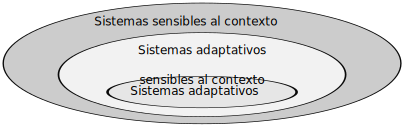
\includegraphics[scale=1]{ContextAwareSystems}
\caption{Sistemas adaptativos sensibles al contexto}
\label{AdaptiveContextAwareSystems}
\end{figure}

\emph{Efstratiou}, continúa detallando que ``se espera que una aplicación adaptativa sensible al contexto, sea capaz de reaccionar a una variedad de \emph{disparadores contextuales}\footnote{Del inglés ``Contextual triggers''.}''. Además, plantea que ``la interacción de múltiples aplicaciones sensibles al contexto que se adaptan a distintos disparadores de entornos, al interrelacionarse podrían causar inestabilidades y comportamientos no deseados''.

Por último, en su tesis explica como coordinar las diferentes aplicaciones, y como resolver los conflictos entre los distintos intereses que puede disparar cada aplicación. Además plantea como involucrar las preferencias del usuario y promover la extensibilidad.

Por otra parte, en 2008, \emph{Costanza} plantea una postura levemente diferente a la de \emph{Dey}. \emph{Costanza} justifica que ``\emph{la definición de Dey} distingue entre información relevante y no relevante, lo cual es importante cuando se está modelando sistemas de adquisición y razonamiento de contextos'', mientras que su definición ``apunta a formas estructuradas de ver cómo se ve afectado el comportamiento del programa en función del contexto, lo cual debería ser abordado por construcciones de uso general y así ser independiente de los tipos de información de contexto de los cuales depende''\cite[p.~1]{Costanza08}.

\emph{Costanza} propone un paradigma de \emph{Programación Orientada a Contextos} (en adelante COP\footnote{Del inglés ``Context-Oriented Programming''.}). En este paradigma, ``los programas se suelen dividir en \emph{variaciones} (o diferenciales) de comportamiento que pueden ser activadas y combinadas en tiempo de ejecución con alcances bien definidos''. El COP ``se centra en construcciones de programación que habilitan el agrupamiento, el referenciamiento, y la activación/desactivación de capas de variaciones en el comportamiento''. Además presenta a \emph{ContextL} que surge como extensión al \emph{Common Lisp Object System}\footnote{El cual es la extensión del lenguaje Common List que brinda soporte a la Programación Orientada a Objetos (o Object Oriented Programming).}, permitiendo asociar la definición de \emph{clases}, \emph{métodos} y \emph{funciones} a distintas \emph{capas} (o variaciones).

\emph{Chang et al.} continuando por la línea de \emph{Dey} y \emph{Efstratiou}, en el 2007, intuye que una aplicación web necesita adaptarse a sí misma a diferentes contextos de ejecución para garantizar cierta \emph{calidad de servicio} (en adelante QoS\footnote{Del inglés ``Quality Of Service''.})\cite[p.~1]{Chang07}. Específicamente, describe que una \emph{aplicación web sensible al contexto} requiere:
\begin{itemize}
	\item La habilidad de \emph{auto-adaptarse} a los entornos específicos de su implementación.
	\item El potencial de \emph{evolucionar} bajo una forma general, tanto a partir del entorno de ejecución como de la forma de uso.
\end{itemize}

Principalmente, Chang menciona que las ``aplicaciones web son esencialmente distribuidas y heterogéneas'', a partir de que existen 2 lugares en donde se puede realizar el procesamiento: el \emph{cliente} y el \emph{servidor}, y en ambos existen alternativas en cuanto a la tecnología utilizada y el entorno disponible. Como consecuencia de esto, desarrolla ``la descomposición de una aplicación web en componentes que serán utilizados si es que el contexto así lo requiere''. Además detalla que es suficiente con que una aplicación se adapte en el momento de \emph{descargarse al cliente}, descartando así la necesidad de adaptación en tiempo de ejecución.

Hacia comienzos del 2009, \emph{Kapitsaki et al.} prosigue en la investigación de sensibilidad al contexto en combinación con aplicaciones web y descarta que la adaptación al contexto deba realizarse dentro del modelo de negocios. Relacionando la sensibilidad al contexto como una característica más que puede contener un Controlador (del esquema MVC)\cite{Kapitsaki09}.

De esta forma, \emph{Kapitsaki et al.} propone una arquitectura en la que, mediante la composición de un grupo de servicios (o aplicaciones web) que no son sensibles al contexto, permite la adaptación al contexto dejando al controlador como responsable de la relación entre el modelo de negocios y el modelo contextual.

También en 2009, \emph{Fortier et al.} plantea un conjunto de micro-abstracciones, que permiten lidiar con la variabilidad de los modelos sensibles al contexto en dispositivos móviles\cite{Fortier09}.


\section{Motivación}


%Teniendo en cuenta la situación cambiante de los \emph{modelos de negocio} actuales y una aplicación web desarrollada con Continuations, en donde el modelo recibe actualizaciones para adaptarse a los nuevos requisitos del sistema y la interfaz gráfica se expande para soportar pantallas específicas para ciertas situaciones del contexto.

Teniendo en cuenta el estado del arte de las aplicaciones web desarrolladas con continuations, en donde no es posible la utilización de sensores para controlar la aplicación. Y considerando las ventajas en la interacción con el usuario que brindan aquellas aplicaciones que se adaptan al contexto.

%Y considerando que no existe una alternativa que permita a una aplicación web desarrollada con Continuations utilizar la información del contexto del cliente, dado que los modelos existentes para adaptar una aplicación web utilizan un esquema MVC\cite{Challiol06,Fortier07,Challiol08,Kapitsaki09,Fortier09}.

Se propone el desarrollo de una librería, que extienda a una implementación de Continuations, para poder utilizar en el servidor la información provista por los sensores de los distintos clientes.

%Para esto se revisará la subclasificación de \emph{Efstratiou}, y a partir de ella se realizará una implementación de \emph{triggers contextuales} que contemple la modificación del contexto de cada usuario, y realice adaptaciones necesarias.

Para esto se utilizará el concepto de \emph{triggers contextuales} mencionado por \emph{Efstratiou}, y como consecuencia se propondrá una implementación de \emph{aplicación web adaptativa al contexto}.

En la solución propuesta, es necesario contemplar los requisitos de cada linea de investigación y tratar de encontrar el mejor compromiso entre ellas.


\section{Contribuciones}

Las contribuciones que se podrán desprender de esta tesis son:
\begin{itemize}
\item Principalmente, la adaptación de una aplicación web que utiliza continuations al contexto del usuario.
\item En segundo término, un análisis de los patrones de diseño que se utilicen en la realización de la librería.
\item Por último, una comparación de la librería propuesta con las librerías existentes para el esquema MVC.
\end{itemize}

Se esperan estas tres contribuciones antes mencionadas. En primera instancia se trata de proveer una librería de sensiblidad al contexto para las aplicaciones web que utilizan continuations.

Para demostrar la utilidad y funcionalidad de la librería se presentará un caso de ejemplo que adapta la aplicación web al contexto del dispositivo.

La segunda contribución es que la librería sea modificable y extensible. Al realizar un análisis de los \emph{patrones de diseño}\cite{Gamma95} utilizados se podrá entender mejor el modelo planteado.

La última contribución se enfoca en realizar una comparación de la librería propuesta y las alternativas existentes que utilizan el esquema MVC.

El alcance de esta tesis no incluirá:
\begin{itemize}
\item discusión alguna sobre la variante \emph{evolutiva} de la sensibilidad al contexto, que utiliza el análisis de las interacciones del usuario para \emph{deducir} nuevas adaptaciones al contexto;
\item pruebas de rendimiento o performance, dado que la realización de estas desviarían el objetivo de esta tesis, que es demostrar la posibilidad de mezclar las dos lineas.
\end{itemize}


\section{Esquema}

El resto de la tesis se organiza de la siguiente manera: en el \emph{Capítulo 2} se desarrollará con profundidad el concepto de continuations en el marco de las aplicaciones web. Dentro del \emph{Capítulo 3} se introducirán los conceptos esenciales sobre aplicaciones sensibles al contexto necesarios para comprender esta tesis.

En el \emph{Capítulo 4} se describirá la solución propuesta y se analizarán los patrones de diseño utilizados.

Un ejemplo completo será presentado en el \emph{Capítulo 5}, en el cual se mostrará la flexibi\-lidad de la librería en la utilización de sensores. Mientras que el \emph{Capítulo 6} mencionará las extensiones posibles para la librería, además de los límites que ésta posee.

Por último, en las \emph{Conclusiones}, se realizará una breve comparación con otros trabajos semejantes, se mencionarán los resultados de esta tesis, y algunas líneas de investigación que se desprenden de este trabajo.

% Chapter 2

\chapter{Continuations en aplicaciones web}
% Write in your own chapter title
\label{Capitulo 2}
\lhead{Capítulo 2. \emph{Continuations en aplicaciones web}} % Write in your own chapter title to set the page header

%-->
% Explicación teórica (no matematica, ni con scheme) de first-class continuations
% Modificaciones/extensiones a continuations
% Aplicaciones web
%- Inconvenientes cuando falta continuations (con MVC)
%	- Flujo de control
%	- Estado
%- Component como bloque de contrucción
%	- Backtracking
%	- Transacciones
%- Combinación con las nuevas tecnologías
%	- AJAX
%	- Server Push
%-->

%Una de las implementaciones más sencillas de \emph{first-class continuations} es la mencionada por \emph{Hieb et al.}\cite[p.~2]{Hieb90}. Ésta consiste en reemplazar la \emph{pila de llamadas tradicional} por una lista enlazada de registros de activación (ver Figura \ref{ContinuationsActivationRecords}).

%\begin{figure}[ht!]
%\centering
%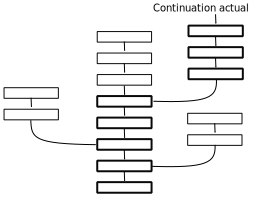
\includegraphics[scale=1]{ContinuationsActivationRecords}
%\caption{Implementación de continuations a partir de una lista enlazada de registros de activación}
%\label{ContinuationsActivationRecords}
%\end{figure}

%En este modelo los registros de activación previamente creados nunca se sobrescriben, y en cambio se crea un nuevo registro por cada llamada. Como contraparte, el adminis\-trador del almacenamiento eliminará un registro en desuso cuando éste ya no pueda ser alcanzado por una \emph{continuation}.

%Existen variantes para esta implementación en las que se desarrollan distintas estructuras de control como \emph{loops}, \emph{nonblind backtracking}\cite{Sussman98}, co-rutinas\cite{Haynes86,Hieb90a,Hieb94}, y engines\cite{Haynes87,Dybvig88} que escapan al alcance de esta tesis.

Como se mencionó en el capítulo anterior, el objetivo de esta tesis es incorporar la información brindada por los sensores de un dispositivo tecnológico en un framework de aplicaciones web basado en continuations.

A partir de esto, es importante destacar que las aplicaciones web desarrolladas con continuations comienzan a surgir en el año 1995. Y gran parte del aporte lo realizaron \emph{Ladd et al.}\cite{Ladd95} y \emph{Quiennec} \cite{Queinnec01}, quienes fueron los primeros en proponer esta variante con el fin de sobrellevar la falta de estado del protocolo \emph{HTTP}\footnote{Del inglés ``Hypertext Transfer Protocol''.}.

% verificar si no queda mejor dado vuelta...

%\emph{Ladd et al.}\cite{Ladd95} y \emph{Quiennec} \cite{Queinnec01} son los primeros en proponer una variante de continuations en el marco de las \emph{aplicaciones web}, para solucionar la falta de estado del protocolo \emph{HTTP}\footnote{Del inglés ``Hypertext Transfer Protocol''.}.

Luego, en el 2004, \emph{Ducasse et al.}\cite{Ducasse04} explica las ventajas de utilizar cierta implementación de continuations para aplicaciones web con respecto a otros frameworks alternativos.

%A continuación se enumeran los \emph{inconvenientes de desarrollar una aplicación web sin continuations}. Luego, se presenta una solución basada en \emph{componentes} reutilizables, que es como Seaside\footnote{Framework para desarrollar aplicaciones web orientado a objetos basado en continuations. Ver \url{http://www.seaside.st/}.} se encuentra implementado actualmente. Por último se describe cómo pueden ser combinadas nuevas tecnologías, como \emph{AJAX}\footnote{Del inglés ``Asynchronous Javascript And XML''.} y \emph{Server Push}\footnote{Técnica que permite enviar información desde el Servidor hacia el Cliente, sin que este último la haya solicitado explícita\-mente.}, con un framework de las características de Seaside.

A continuación se enumeran los \emph{inconvenientes de desarrollar una aplicación web sin continuations}. Luego, como contraparte se presenta Seaside\footnote{Framework para desarrollar aplicaciones web orientado a objetos basado en continuations. Ver \url{http://www.seaside.st/}.}, una solución basada en continuations a partir de \emph{componentes} reutilizables, ampliamente utilizada por los desarrolladores de aplicaciones web.

%Por último, dado que Seaside va a ser el framework en donde se realizarán las pruebas pertinentes, se describirá como ha sido extendido para soportar funcionalidades como \emph{AJAX}\footnote{Del inglés ``Asynchronous Javascript And XML''.} y \emph{Server Push}\footnote{Técnica que permite enviar información desde el Servidor hacia el Cliente, sin que este último la haya solicitado explícita\-mente.}, que son técnicas utilizadas en gran parte de las aplicaciones web de la actualidad.
Por último, y considerando que Seaside va a ser el framework en donde se realizarán las pruebas pertinentes, se describirá como ha sido extendido para soportar funcionalidades como \emph{AJAX}\footnote{Del inglés ``Asynchronous Javascript And XML''.} y \emph{Server Push}\footnote{Técnica que permite enviar información desde el Servidor hacia el Cliente, sin que este último la haya solicitado explícita\-mente.}, que son técnicas utilizadas en gran parte de las aplicaciones web de la actualidad.


\section{Inconvenientes de los frameworks sin continuations}

Al desarrollar aplicaciones web con frameworks que no se basan en continuations existen un conjunto de inconvenientes y/o contratiempos que deben ser resueltos. Algunos de ellos consecuencia de una escasa abstracción sobre el protocolo HTTP, y otros por restricciones planteadas por el esquema REST\cite[p.~76]{Fielding00} existente en muchos frameworks.

%Como sintetiza \emph{Ducasse et al.}\cite[p.~234]{Ducasse04} existen dos tipos de dificultades cuando se utilizan la mayoría de los frameworks actuales (tales como Struts\footnote{\url{http://struts.apache.org/}}, Symfony\footnote{\url{http://www.symfony-project.org/}}, ASP.net\footnote{\url{http://www.asp.net/}}, Rails\footnote{\url{http://rubyonrails.org/}}, etc.): los relacionados con la lógica del \emph{flujo de control} y los que conciernen al \emph{estado} entre las interacciones del usuario.

Como sintetiza \emph{Ducasse et al.}\cite[p.~234]{Ducasse04} existen dos tipos de dificultades cuando se utiliza algún framework alternativo (tal como Servlets/JSP\footnote{\url{http://java.sun.com/products/servlet/} y \url{http://java.sun.com/products/jsp/}}, PHP\footnote{\url{http://www.php.net/}}, ASP\footnote{\url{http://msdn.microsoft.com/en-us/library/ms972347.aspx}}, JSP\footnote{\url{http://java.sun.com/products/jsp/}} o Zope\footnote{\url{http://www.zope.org}}): los relacionados con la lógica del \emph{flujo de control} y los que conciernen al \emph{estado} entre las interacciones del usuario.


\subsection{Flujo de control}

Al considerar el flujo de control de estos últimos frameworks, se observa que fallan en proporcionar una abstracción de alto nivel para especificar cómo son enlazadas las páginas.

La lógica del flujo de control debería estar implementada idealmente en una única porción de código, que utilice estructuras de control comunes al lenguaje de programación utilizado para especificar el modelo de negocios. Desafortunadamente, esta forma de programar es opuesta a lo que el protocolo HTTP establece (con sus mensajes de solicitud y respuesta).

Los problemas más relevantes relacionados con el flujo de control son:

\begin{description}

\item[Mezclar la lógica de aplicación con la lógica de los componentes.]

La interacción del usuario en una aplicación web puede ser vista como dos tareas que se repiten en el tiempo: la primera es \emph{generar la página} y la segunda \emph{procesar los datos} cuando el usuario los envíe. Estas tareas se ejecutan de forma separada y levemente conectadas.

De esta forma, la decisión de \emph{``¿qué es lo que hago a continuación?''} está asociada a la parte de procesamiento de datos de la última página, en lugar de ser definido como un \emph{flujo de control} a más alto nivel.

En los frameworks orientados a páginas cada componente debe indicar como interactúa con el resto. Así, cada página en una secuencia tendrá un enlace \emph{estructurado de forma estática}\footnote{Traducción no literal de ``hardcoded''.} a la próxima.

\item[Incapacidad para componer flujos de control.]

No todos los frameworks para desarrollar aplicaciones web proveen la capacidad de reutilizar componentes (en donde cada uno posee su propio flujo de control). Esto dificulta la posibilidad de trabajar con \emph{múltiples flujos de control} en una misma página.

\item[Controlar el flujo del programa.]

Dado que el usuario puede clonar una página e ir hacia atrás en el historial, es necesario contar con la posibilidad de \emph{invalidar} un flujo de control luego de que una \emph{transacción} se haya concluido y aceptado.

\end{description}


\subsection{Estado}
\label{ControlFlowStates}

Por otra parte, una aplicación web típica tiene que tratar con tres tipos de estados: el asociado a la \emph{interfaz gráfica con el usuario} (de cada componente), el del \emph{modelo del dominio} (relacionado con las instancias del modelo del negocio) y el referido a la \emph{sesión de usuario} (se encarga de mantener estados globales de la sesión, que no pertenecen al modelo de negocios ni a la interfaz gráfica con el usuario). Un ejemplo de este ultimo tipo de estado es la identificación del usuario, que suele ser común a todos los componentes.

Pero administrar el estado en el ámbito de una aplicación cliente-servidor es complejo como consecuencia del flujo de control no lineal. Esto, principalmente, es causado por la incapacidad del protocolo HTTP de mantener estados y por las capacidades de los navegadores web (clonar y/o retroceder).

Actualmente, en los frameworks orientados a páginas el estado es codificado en las respuestas al cliente. Esta solución temporal conduce a los siguientes inconvenientes:


\begin{description}

\item[Codificar el estado.]

Cuando el estado del modelo del dominio debe ser tenido en cuenta sobre una secuencia de páginas, cada página tiene que pasar la información recibida desde las páginas anteriores y trasladarla a la próxima. Esto produce que el código no sea reutilizable por su dependencia de las páginas precedentes.

\item[Colisión de los nombres.]

Puede haber colisiones en los nombres de las \emph{URL}\footnote{Del inglés ``Uniform Resource Locator''.} o en los campos de los formularios. El programador debe encargarse de que los identificadores sean únicos a lo largo de una página. Esto se vuelve especialmente un problema cuando se desean reutilizar los componentes.

\item[Mezclar la lógica de presentación con la del dominio.]

Para codificar el estado en una página se deberá mezclar la generación de HTML\footnote{Del inglés ``Hypertext Markup Language''.} con la lógica de dominio usando \emph{templates} o la concatenación de \emph{strings}. Esto terminará produciendo código fuente difícil de leer.

\end{description}


\section{El \emph{Componente} como bloque de construcción}

A partir de los inconvenientes planteados con el flujo de control y la administración de estados, existen frameworks como Seaside en los que se propone la construcción de una página a partir de \emph{componentes}\footnote{Seaside lo implementa en la clase \emph{WAComponent}.}. Cada componente se encarga de definir la interfaz de usuario y el flujo de control de una parte de la aplicación. A diferencia de los frameworks orientados a páginas la instancia de un componente a menudo perdura a lo largo de la sesión del usuario.

En cada solicitud el framework le permite a cada componente evaluar sus \emph{callbacks} y \emph{renderizar} su estado actual en un \emph{stream de respuesta}.

Las características más importantes de esta aproximación son: el \emph{renderizado}, la \emph{composición de componentes} y los \emph{action callbacks}.

\begin{description}

\item[Renderizado.]

Cada componente que es visible en una aplicación web tiene un \emph{método de enganche}\footnote{Del inglés ``callback''.}, que permite definir su aspecto visual. Este método es llamado con un \emph{stream de respuesta} como parámetro, permitiendo especificar las características gráficas y de comportamiento de cada componente con el mismo lenguaje en el cual está implementado el modelo de negocios.

\item[Composición de componentes.]

Para la construcción de una aplicación web un componente puede contener a muchos otros. De esta forma una ``página'' sería definida como un componente compuesto. Por otra parte existe un componente específico denominado \emph{Task}, que se encarga solamente de definir un flujo de control, y así prescindir del \emph{renderizado}.

\item[Action Callbacks.]

Los componentes pueden reaccionar a las acciones realizadas por el usuario a través de los \emph{action callbacks}. Estos son definidos sobre los \emph{botones}, \emph{enlaces} y por cada campo de un formulario mediante la utilización de un \emph{bloque de código o functor} al momento de describir el comportamiento de un componente.

El \emph{action callback} de un campo del formulario contiene un argumento que representará al valor del campo en cuestión. Mientras que para los enlaces y botones el bloque no contiene ningún argumento, en estos se define el flujo de control del componente o de la aplicación.

\end{description}

Dado que cada componente define su propio flujo de control independiente de los otros mostrados en la misma página, un componente o aplicación puede tener múltiples flujos de control.

Cada vez que el usuario utilice un \emph{enlace} o un \emph{botón} en un componente realizará un paso hacia adelante en su flujo de control, mientras el resto de los flujos de control permanecen en el mismo estado.

Para facilitar la creación y administración de múltiples flujos de control los frameworks basados en \emph{componentes} proporcionan los métodos \textbf{call:} y \textbf{answer:}.

\begin{description}

\item[Call.]

Mediante este método un componente (por ejemplo \emph{A}) puede pasarle el control a cualquier otro componente (en este caso \emph{B}). Durante este tiempo el componente original (\emph{A}) es temporalmente reemplazado por el otro componente (\emph{B}). Esto es posible mediante el envío del mensaje \textbf{call:} al componente \emph{A} y enviándole como parámetro el componente \emph{B}.

\item[Answer.]

Mediante este método un componente (por ejemplo el \emph{B}) puede devolver el control a aquel componente desde el cual ha sido llamado (en este caso el \emph{A}). Cada componente eventualmente devolverá el control de la ejecución en algún punto, e inclusive puede retornar un objeto que modele la respuesta. Esto es posible mediante el envío del mensaje \emph{answer:} al componente \emph{B} y enviándole como parámetro el objeto que modela la respuesta.

\end{description}

Aunque desde la perspectiva del desarrollador el código es lineal, existen algunas cuestiones relacionadas con el estado de la aplicación web que deben ser explicadas.

Seaside permite la \emph{clonación} de una página y \emph{volver} al estado anterior. De esta forma es necesario que exista cierto mecanismo que se encargue de mantener el estado de la \emph{interfaz gráfica} y del \emph{modelo del dominio}, ambos mencionados en la sección \nameref{ControlFlowStates} (\ref{ControlFlowStates}).


\subsection{Backtracking}

Dado que cada componente tiene su propio estado, el cual es guardado en las variables de instancia (por ejemplo un componente que muestra un listado de elementos de forma paginada recordará el numero de la página actual). Cuando el usuario \emph{vuelve} hacia atrás con el navegador web, las variables de instancia del componente pueden no representar el estado que el usuario visualiza.

Una forma de mantener el estado de los componentes en sincronía con lo que visualiza el navegador web es mediante la utilización de continuations. Para esto, Seaside ofrece un mecanismo para seleccionar qué variables de instancia deben ser \emph{rastreadas}\footnote{Del inglés ``backtracking''.}. Después de cada respuesta enviada al cliente, el framework guarda una copia exacta de los objetos seleccionados mediante la creación de un \emph{registro de activación}.

La sesión del usuario almacena el registro como una variable temporal dentro del proceso que envía la \emph{respuesta} al cliente y que luego recibirá la próxima \emph{solicitud}. El registro se vuelve persistente hasta un momento en el futuro en el cual el flujo de control requiera retomar la ejecución de este componente almacenado.

Al momento de restablecer el \emph{contexto de ejecución} y antes de procesar la solicitud del cliente, el registro restablece los objetos registrados y la \emph{continuation} es procesada.

Esto asegura que cuando se procesa una solicitud, los valores son los mismos que cuando la respuesta previa fue creada.


\subsection{Transacciones}

En ciertas aplicaciones complejas suele ser necesario interceder para prevenir que el usuario retroceda a la página anterior. Seaside implementa el método ``\emph{isolate: aBlockClosure}'' para controlar el flujo de control. Este método recibe un \emph{bloque de código} o \emph{functor} como argumento, el cual es tratado como una transacción.

La transacción le garantiza al usuario poder ir hacia adelante y hacia atrás, siempre y cuando permanezca dentro del \emph{bloque transaccional}. Sin embargo, una vez terminada la transacción el usuario no podrá volver hacia atrás, dado que la transacción ha sido dada por concluida.


\section{Combinación con las nuevas tecnologías}

Al considerar el requisito de extender una aplicación web basada en continuations, es necesario corroborar como se han realizado otras extensiones al framework presentado.

Para esto, a continuación se repasará como otras librerías de terceros han incorporado dos protocolo de comunicación como \emph{AJAX}\footnote{Es la sigla de ``Asynchronous Javascript And XML''.} y \emph{Server Push} al framework Seaside.


\subsection{Asynchronous Javascript And XML}

El uso masivo de las aplicaciones web comienza a evidenciar que las interacciones del usuario se realizan sobre ciertas partes de una página, mientras que otras partes permanecen inalteradas.

Como consecuencia se comienza a trabajar en una abstracción que permita desacoplar la interacción del usuario de la carga de la página, con el fin que puedan realizarse solicitudes de forma asíncronas y manipular las respuestas para que puedan ser incluidas en la porción de página que debe ser actualizada.

Esta abstracción es denominada \emph{AJAX} y es totalmente compatible con el protocolo HTTP, dado que mantiene el requisito que una \emph{respuesta} del servidor solo será dada a partir de una \emph{solicitud} del cliente\footnote{Detallado en la \emph{RFC2616} (\url{http://www.ietf.org/rfc/rfc2616.txt}).}.

% Se denomina \emph{AJAX} a la abstracción que brinda la posibilidad de que el navegador web realice solicitudes de forma asíncronas al servidor, sin la necesidad de recargar toda la página. Así, la información recibida es utilizada para actualizar sólo una porción de la página. Esta técnica es totalmente compatible con el protocolo HTTP, dado que mantiene el ciclo de solicitud/respuesta\footnote{Detallado en la \emph{RFC2616} (\url{http://www.ietf.org/rfc/rfc2616.txt}).}.

Para soportar \emph{AJAX} de una forma transparente al desarrollador, Seaside agrega la clase \emph{SUComponent} que es una especialización del \emph{WAComponent}\footnote{Componente base del framework Seaside.} (ver Figura \ref{SUComponent}).

\begin{figure}[ht!]
\centering
\includegraphics[scale=1]{SUComponent}
\caption{Extensión de Seaside para soportar AJAX}
\label{SUComponent}
\end{figure}

El componente \emph{SUComponent} es una implementación del patrón \emph{Abstract Factory}\cite{Gamma95} que permite la creación de objetos \emph{SUAjax}.

Cada instancia de \emph{SUAjax} representa una posible solicitud asíncrona que puede realizar el cliente. Luego, en el momento del \emph{renderizado}, el framework podrá procesar la respuesta que posteriormente será enviada al cliente.


\subsection{Server Push}

La utilización de AJAX dio lugar a un nuevo conjunto de aplicaciones web que mejoran la interacción e intercomunicación entre distintos usuarios.

Para esto un navegador web debe preguntar al servidor de forma periódica si existen actualizaciones para cierto usuario. Cuanto mas seguido pregunta, más interactiva se vuelve la aplicación. Aunque existen ciertas aplicaciones web en donde el cliente consulta muchas veces y las actualizaciones son por momentos pocas y por momentos muchas.

Esto planteó otra situación, y es que los navegadores solo pueden obtener las actualizaciones de los otros usuarios a partir de solicitarlas al servidor, como consecuencia del ciclo solicitud/respuesta del protocolo HTTP.

Para mejorar esto, \emph{Server Push} utiliza conexiones \emph{HTTP} de larga duración para reducir la \emph{latencia} de comunicación entre el \emph{servidor web} y el \emph{navegador}. Esto implica una \emph{optimización} con respecto a AJAX, al permitir que un servidor inyecte información en un cliente en particular.

Desde el punto de vista del cliente, en lugar de solicitar reiteradamente al servidor por la existencia de alguna actualización, el navegador deja una conexión abierta\footnote{Conceptualmente se considera que es una conexión abierta, aunque en realidad se suele utilizar un \emph{timeout} elevado que eventualmente podrá cerrar la conexión.}. De esta forma el servidor cuenta siempre con un canal para enviar información, teniendo la capacidad de establecer el momento en el que el cliente recibirá la información.

Para implementar \emph{Server Push}, \emph{Seaside} agrega la clase \emph{Meteoroid} que es una especiali\-zación del \emph{WAComponent} (ver Figura \ref{Meteoroid}).

\begin{figure}[ht!]
\centering
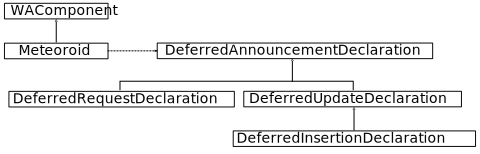
\includegraphics[scale=1]{Meteoroid}
\caption{Extensión de Seaside para soportar Server Push}
\label{Meteoroid}
\end{figure}

El componente \emph{Meteoroid} permite actualizar el contenido del cliente web mediante tres acciones: una \emph{solicitud}, la \emph{inserción} y la \emph{actualización}.

La \emph{solicitud} posibilita que el servidor obligue al cliente a realizar una \emph{solicitud asíncrona mediante AJAX}.

Por otra parte, mientras la \emph{inserción} siempre agrega el contenido al final de una \emph{etiqueta HTML}, la \emph{actualización} reemplaza el contenido completo.

% Chapter 3

\chapter{Sensibilidad al contexto}
% Write in your own chapter title
\label{Capitulo 3}
\lhead{Capítulo 3. \emph{Sensibilidad al contexto}} % Write in your own chapter title to set the page header

Luego de describir a Seaside como referente para desarrollar aplicaciones web basadas en continuations, es necesario explicar que alternativas existen para procesar la información provista por un conjunto de sensores.

Una forma de organizar la utilización de sensores es mediante el concepto de \emph{sensibilidad al contexto}.

Para poder definir la sensibilidad al contexto es necesario repasar que significa \emph{contexto}, \emph{entorno} y \emph{adaptación}; para luego poder definir la \emph{sensibilidad al contexto}.

%Para comprender la sensibilidad al contexto es importante entender algunos conceptos básicos como el \emph{contexto}, el \emph{entorno} y la \emph{adaptación}.

La primera definición de \emph{contexto}, que es la más adoptada, es la que aporta \emph{Dey} en 2001, que estipula:

\begin{quote}
Contexto es cualquier información que pueda ser usada para caracterizar la situación de una entidad.\cite[p.~3]{Dey01}
\end{quote}

Por su parte, \emph{Dourish} intenta destacar una característica dinámica al intentar abstraer al contexto y en 2004 afirma:

\begin{quote}
Contexto es un concepto de lo que se mantiene al margen, y se disuelve cuando uno intenta definirlo.\cite{Dourish04}
\end{quote}

De esta forma \emph{Dourish} destaca lo complejo que es definir un modelo para representar al contexto, dado que cierta información del contexto puede transformarse en información del modelo y viceversa. Además, presenta un modelo contextual basado en interacciones, que se enfoca en responder ``¿cómo y por qué las personas mantienen un entendimiento mutuo del contexto en el curso de las interacciones de sus acciones?''; evitando así la definición de un contexto \emph{estable} y \emph{delineable} en tiempo de implementación\cite[p.~5]{Dourish04}.

Por otra parte, el \emph{entorno} es la caracterización de las circunstancias de una situación en particular combinado con la descripción de la adaptación a realizarse para mejorar la interacción con el usuario de ese contexto. Es el punto de conexión entre un modelo de negocios y el modelo del contexto, que se encarga de describir ante qué circunstancias se realiza cierta \emph{adaptación}.

Luego, la \emph{adaptación} consiste en realizar un conjunto de acciones de forma automática para simplificar la interacción de una entidad con uno o varios sistemas. Aunque estas acciones sólo afectarán al modelo de negocio, se debe tener en cuenta que cierta información del contexto puede transformarse en información del modelo de negocio y viceversa.

A partir de estos conceptos, se considera que la \emph{sensibilidad al contexto} es una característica de los sistemas que simplifica la interacción con un usuario (o entidad) a partir del \emph{entendimiento} de la situación del mismo (o la misma). Ese \emph{entendimiento} está determinado por la capacidad de un sistema de identificar un \emph{entorno} y luego proporcionar una \emph{adaptación}.

A continuación, dado que la sensibilidad al contexto se encuentra estrechamente relacionada con los sistemas adaptativos, se definen a las \emph{aplicaciones adaptativas sensibles al contexto} de \emph{Efstratiou}\cite{Efstratiou04} para delinear el alcance de esta tesis. Luego, se introducen los conflictos que existen cuando se procede a combinar la sensibilidad al contexto con un framework de aplicaciones web basado en continuations.


\section{Aplicaciones adaptativas sensibles al contexto}

Los sistemas adaptativos\cite{Cen97,Kokar99,Meng01} están basados en la teoría del \emph{control mediante la retroalimentación}\footnote{Utilizado por primera vez en la ingeniería electrónica.} (ver Figura \ref{FeedbackControlSystem}).

\begin{figure}[ht!]
\centering
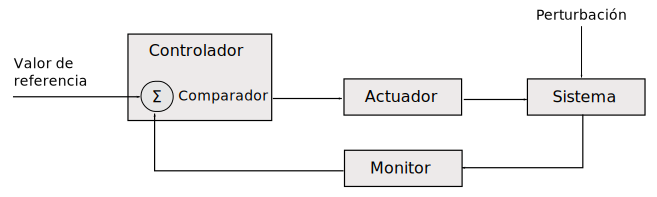
\includegraphics[scale=0.75]{FeedbackControlSystem}
\caption{Sistema de control mediante la retroalimentación}
\label{FeedbackControlSystem}
\end{figure}

El \emph{controlador}\footnote{Este es el \emph{controlador} de la adaptación y no se encuentra directamente relacionado con el controlador del MVC.} se encarga de mantener el valor de referencia de una variable de control, mientras reduce la sensibilidad del sistema a posibles perturbaciones. El controlador interactúa con el sistema a través de \emph{monitores} y \emph{actuadores}.

Un monitor mide la variable controlada, y es la fuente de retroalimentación. La salida del controlador causa que el actuador realice la adaptación al comportamiento del sistema en respuesta a las perturbaciones (o cambios en el entorno).

La abstracción de este sistema puede sintetizarse en un \emph{ciclo de adaptación básico} (ver Figura \ref{BasicAdaptationCycle}) que incluye los siguientes elementos funcionales:

\begin{figure}[ht!]
\centering
\includegraphics[scale=0.75]{BasicAdaptationCycle}
\caption{Ciclo de adaptación básico}
\label{BasicAdaptationCycle}
\end{figure}

\begin{description}
\item[Monitor:] El primer elemento realiza el monitoreo de una fuente de información específica que es \emph{interesante} para el mecanismo de adaptación. Esta fuente de información puede estar determinada por la disponibilidad de un recurso específico o un \emph{disparador contextual} que notifique la ocurrencia de un evento.
\item[Controlador:] El segundo elemento es el mecanismo de control que toma las decisiones necesarias para adaptarse al entorno. Esta decisión se basa en la información recibida por el monitor.
\item[Actuador:] El tercer elemento es el encargado de realizar la adaptación mediante la ejecución de acciones correctivas, a medida que el controlador lo disponga. La conexión entre el actuador y el recurso que está siendo monitoreado no necesariamente existe en todos los sistemas.
\end{description}

\emph{Efstratiou}\cite{Efstratiou04} destaca que una \emph{aplicación adaptativa} adquiere la característica de ser \emph{sensible al contexto} cuando la información a ser monitoreada, en lugar de provenir de un recurso específico, proviene del \emph{contexto externo} de la aplicación (cualquier porción de información que actualmente no pertenezca al \emph{modelo de negocio}).


\section{Conflictos entre la sensibilidad al contexto y las aplicaciones web desarrolladas con continuations}
\label{Conflictos entre sensibilidad y aplicaciones web}

Al comenzar a combinar las aplicaciones web basadas en continuations con técnicas utilizadas por las aplicaciones adaptativas sensibles al contexto surgen dos situaciones de conflicto: la \emph{privacidad} y las \emph{transacciones con adaptación al contexto}.


\subsection{Privacidad}

Las \emph{aplicaciones web} se ejecutan encapsuladas en el navegador web para proveer de cierta seguridad y privacidad al usuario. Se intenta separar su información privada y el conjunto de dispositivos conectados a una computdadora de las inseguridades que provee una conexión a Internet (o intranet).

Por otra parte las \emph{aplicaciones adaptativas sensibles al contexto} necesitan el acceso a la información privada del usuario y a un conjunto de sus sensores, con el fin de identificar el contexto (o entorno) de forma automática y promocionar adaptaciones que simplifiquen la actividad cotidiana del usuario.

Ante esta situación conflictiva, en donde una de las partes restringe el acceso al sistema y la otra requiere todo lo contrario para funcionar, es importante presentar una solución intermedia que brinde la información suficiente para la adaptación, siempre y cuando el usuario lo desee. En el mas restrictivo de los escenarios, el usuario terminará utilizando una aplicación web convencional en donde no exista sensibilidad al contexto.


\subsection{Transacciones}

Las aplicaciones web basadas en continuations suelen contener flujos de control con soporte para transacciones. Una transacción garantiza que un conjunto de acciones sean ejecutadas de forma consecutiva, y ante algún inconveniente existe un mecanismo de \emph{restauración} para dejar el sistema en el estado previo.

Las transacciones son utilizadas por aplicaciones con ejecuciones concurrentes, en donde se desea evitar la corrupción o inconsistencia de los datos al ser persistidos.

Como contraparte, en las aplicaciones adaptativas, las acciones son ejecutadas a partir de una necesidad de adaptación de un sistema a un contexto dado. Una acción siempre depende del entorno que motivó la adaptación.

En las aplicaciones adaptativas la persistencia de la información suele ser realizada de forma acumulativa, de tal manera que se memorice el progreso de la adaptación a través del tiempo. A partir de estos datos, un sistema evolutivo podría reconocer nuevos patrones de comportamiento de un usuario, y proveer nuevas adaptaciones.

Esto produce que no se necesiten modificar valores previos en los sistemas adaptativos, descartando en gran medida la necesidad de transacciones.

El conflicto entre ambas partes ocurre cuando una transacción de un sistema basado en continuations falla y se desea restaurar el sistema a una versión previa. En los sistemas adaptativos sensibles al contexto la única interpretación que admitiría restablecer los registros a un estado previo es aquella que se produciría si se pudiese retroceder el tiempo y sus consecuentes estados.

Dado que esto es improbable, resulta necesario contemplar una alternativa que permita mezclar las transacciones de continuations con la ``progresividad'' de la sensibilidad al contexto.

Para evitar esta situación, se descarta el análisis de cualquier variante \emph{evolutiva} de sensibilidad al contexto en donde se requiere de este tipo de persistencia y se opta por integrar la adaptación al contexto sobre el framework que administra las continuations.

Esto significa que Seaside, administrará las transacciones (encargandose del estado correspondiente) y luego la sensibilidad al contexto por sobre Seaside reconocerá entornos y le notificará al framework para que ejecute las acciones de adaptación correspondiente.

Estas ejecuciones asociadas a ciertos entornos, podrán deshacerse fácilmente al no persistirse la información perteneciente a la sensibilidad al contexto. Solo se persistirán las consecuencias de las adaptaciones en el modelo de negocio de la aplicación transaccional.

% Chapter 4

\chapter{Diseño}
% Write in your own chapter title
\label{Capitulo 4}
\lhead{Capítulo 4. \emph{Diseño}} % Write in your own chapter title to set the page header

%Al considerar los objetivos planteados en la introducción y los conflictos planteados en el capítulo anterior, surge la necesidad de desarrollar una alternativa que incorpore la sensibilidad al contexto a las aplicaciones web desarrolladas con continuations.
Al considerar los objetivos planteados en la introducción, que promueven la incorporación de la sensibilidad al contexto a las aplicaciones web desarrolladas con continuations, y los conflictos planteados en el capítulo anterior; surge la necesidad de diseñar una abstracción que busque una buena relación entre la sensibilidad al contexto y la privacidad del usuario.

La alternativa propuesta en esta tesis consiste en la creación de una librería que permita conocer el estado de los sensores del cliente desde el servidor, manteniendo la capacidad \emph{transaccional} de las aplicaciones web basadas en continuations, a la vez que se intenta mantener la \emph{privacidad del usuario} proporcionada por los navegadores web convencionales.

A continuación se detallan las decisiones de diseño tomadas comenzando desde el navegador web y culminando en el servidor. Primero se analizará la \emph{privacidad del usuario} en el cliente. Luego se prosigue con el \emph{mecanismo de suscripción/notificación en el cliente}, para posteriormente explicar el mismo \emph{mecanísmo visto desde el servidor}.

Por último se describe el proceso necesario para \emph{brindar soporte a un nuevo sensor}, y se presenta el \emph{modelo final}.


\section{Privacidad del usuario}

La privacidad del usuario de una aplicación web se encuentra determinada tanto por los navegadores web, como por la forma en que fue desarrollada esa aplicación.

La privacidad proporcionada por los navegadores web convencionales, consiste en aislar la ejecución de la aplicación web de una gran cantidad de información disponible en un dispositivo (como archivos, otros dispositivos conectados, sensores, etc).

Por otro lado, dado que la sensibilidad al contexto requiere información específica del usuario, es necesario acceder a cierta información protegida por la mayoría de los navegadores web (valores de los sensores que permitan reconocer el entorno del dispositivo, y a su vez parte del entorno del usuario).

Una forma de permitir el acceso a esta información desde las aplicaciones web se logra al proporcionar una API\footnote{Del inglés ``Application Programming Interface''.} que acceda a los valores de los sensores. Además, el navegador web, deberá proporcionar una interfaz para que el usuario pueda establecer a que información puede acceder la aplicación web.

Por ejemplo, el navegador web utilizado para la realización de esta tesis\footnote{Construido como consecuencia de la escasez de este tipo de navegadores web.}(basado en Phonegap) al presionar la tecla menú (en un dispositivo móvil) muestra una lista de sensores, desde donde se podrá seleccionar cuales serán compartidos mediante la API (Ver Figura \ref{PhoneGapBrowserLike}).

\begin{figure}[ht!]
\centering
\framebox[2.01in]{
\noindent
\includegraphics[scale=0.3]{Screenshot_2012-06-03-01-43-29}
}
\caption{Captura de pantalla del navegador web Phonegap}
\label{PhoneGapBrowserLike}
\end{figure}

Luego, dentro de las aplicaciones web, las interfaces (disponible desde Javascript) dependen de la velocidad con que se actualiza la información del sensor.

Aquellos sensores que recuperan información altamente cambiante (como el acelerómetro, el compás y la posición) proporcionan una interfaz para configurar un \emph{timer}\footnote{Tarea que se ejecuta de forma reiterativa dado cierto intervalo de tiempo.} mediante una función que requiere de 3 parámetros (ver Figura \ref{PhonegapAPI}, linea 4).

\begin{figure}[ht!]
\begin{Verbatim}
succes = function (listened) { };
fail = function (error) { };
options = { frequency: 1000 };
timerId = navigator.geolocation.watchPosition( sucess , fail , options );
\end{Verbatim}
\caption{Ejemplo de API en el lenguaje javascript para los sensores altamente cambiantes}
\label{PhonegapAPI}
\end{figure}

Los 2 primeros parmámetros son \emph{callbacks} (ver lineas 1 y 2) y el último un diccionario con \emph{opciones} de configuración (ver linea 3). El primer callback se ejecuta cuando se ha podido obtener la información de forma correcta, y el  otro en caso de que el sensor se haya encontrado con algún inconveniente.

Por otra parte, aquellos sensores que recuperan información menos dinámica (como la batería, la red a la que se encuentra conectado, etc.) suelen proveer una función para solicitar el valor actual.

Estas herramientas proporcionadas por el navegador web para que el usuario pueda seleccionar que parte de su contexto desea compartir son una parte de la solución al problema de la privacidad. La otra parte de la solución se encuentra en la forma que se encuentra desarrollada la aplicación web.

Si se tiene en cuenta la privacidad del usuario al momento de diseñar una aplicación web, existen ciertas decisiones de diseño que pueden ser tomadas.

Un aspecto importante de la privacidad del usuario, es reducir al mínimo la transferencia de información de los sensores hacia los servidores, comunicando solo aquella información que sirva para tomar una decisión en el servidor.

Este tipo de optimización, puede ser realizada al utilizar el patrón de diseño \emph{Publish/Subscriber} descripto por \emph{Birman et al.}\cite{Birman87}, que permite registrarse a un entorno de interés, en lugar de requerir que el cliente envíe el estado de sus sensores de forma continua.

De esta forma, el servidor deberá registrarse a un entorno determinado (mediante algún mecanismo de \emph{Server Push}) y el cliente realizará la notificación pertinente cuando el entorno sea compatible con el contexto del usuario.


\section{Mecanismo de suscripción a un entorno}

Para realizar una suscripción a un entorno, es necesario diseñar una estructura que detalle las características que permiten describirlo.

Hay entornos que dependen de la información de un solo sensor, mientras que existirán otros que dependen de una combinación de varios. Inclusive, sería deseable, que se puedan definir \emph{sub-entornos} que luego puedan ser reutilizados en diferentes entornos mas complejos.

Para obtener esta \emph{granularidad} en la definición del entorno, se utiliza el patrón de diseño \emph{Composite} descripto por \emph{Gamma et al.}\cite{Gamma95}, mediante las clases \emph{Condition}, \emph{SimpleCondition} y \emph{ComplexCondition} (ver Figura \ref{CompositeCondition}).

\begin{figure}[ht!]
\centering
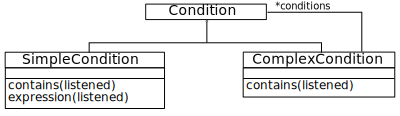
\includegraphics[scale=1]{ConditionComposite}
\caption{Implementación del patrón Composite mediante la clase Condition}
\label{CompositeCondition}
\end{figure}

La clase \emph{SimpleCondition} representa al estado deseado de un sensor en un momento determinado. Es la menor granularidad posible dentro de la definición del entorno, pudiendo evaluarse si el estado de un sensor cumple con su requisito mediante el método \emph{contains}.

Por otra parte, la clase \emph{ComplexCondition} permite la caracterización de entornos a partir de la utilización de varios sensores. Cuando se evalúa una condición compleja (utilizando el método \emph{contains}) se tiene en cuenta que todas las condiciones que la componen se cumplan. En caso de no cumplirse alguna de las condiciones, la condición compleja tampoco se cumplirá.

Por último, para homogeneizar las distintas interfaces (o API) con las que se puede acceder a la información de un sensor (mediante el patrón de diseño \emph{Adapter}\cite{Gamma95}), se crea la clase \emph{Listener} que abstrae a las \emph{SimpleCondition} de la API específica del Phonegap (ver Figura \ref{ListenerAbstraction}).

\begin{figure}[ht!]
\centering
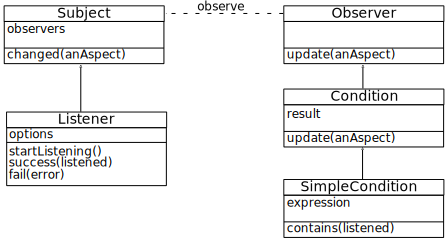
\includegraphics[scale=1]{ListenerAbstraction}
\caption{Abstracción de los sensores mediante la clase Listener}
\label{ListenerAbstraction}
\end{figure}

Dentro de una instancia de la clase \emph{Listener}, el método \emph{startListening} se encargará de inicializar un \emph{timer} (o, dependiendo del caso, de configurar el \emph{timer} perteneciente a la API de Phonegap) que será el encargado de leer el valor. En caso de éxito se llamará al método \emph{success} y en caso de error al método \emph{fail}.

Cada instancia de \emph{SimpleCondition} observará (mediante el patrón de diseño \emph{Observer} presentado por \emph{Gamma et al.}\cite{Gamma95}) a una instancia de la clase \emph{Listener}. De esta forma, cuando un \emph{Listener} conozca una nueva lectura de su sensor, las \emph{SimpleCondition} que lo observan podrán actuar al respecto.

Este proceso se encuentra detallado dentro del método \emph{success} de la clase \emph{Listener} en donde se notifica a cada \emph{SimpleCondition} que se encuentra observando, utilizando el método \emph{update}. Dentro de \emph{update}, cada \emph{SimpleCondition} evaluará si contiene (utilizando el método \emph{contains}) al valor informado por el sensor.

Una vez definidas las clases que permitirán la descripción y detección del entorno, es necesario detallar el mecanismo de notificación al servidor.


\section{Notificación al servidor de la ocurrencia de un entorno}

Teniendo en cuenta que el servidor se suscribió a un entorno detallado (descrípto por un conjunto de condiciones), cuando el cliente realice la notificación no requerirá el envío de información sobre el entorno.

El cliente solo informará cual es el \emph{callback de continuations} que el servidor debe ejecutar mediante una solicitud \emph{AJAX}, la cual ha sido administrada por el servidor al momento de registrarse al cliente. El cliente guarda dicha solicitud de forma \emph{serializada} en el atributo \emph{callback} de la clase \emph{Trigger}.

Luego, una instancia de la clase \emph{Trigger} se relaciona con una instancia de la clase \emph{Condition}, quedando asociado la descripción de un entorno determinado con una notificación al servidor (ver Figura \ref{TriggerNotification}).

\begin{figure}[ht!]
\centering
\includegraphics[scale=1]{TriggerNotification}
\caption{Implementación de la clase Trigger como parte escencial del patrón Public/Subscriber}
\label{TriggerNotification}
\end{figure}

Notar que la clase \emph{Condition} además de ser un \emph{observador} es un \emph{subjeto}, a partir de esto podrá ser observada por una instancia de la clase \emph{Trigger} o por una instancia de \emph{ComplexCondition}.

De esta forma, cuando la clase \emph{Listener} recupera un nuevo valor del sensor, se lo notifica a todas las \emph{SimpleCondition} que lo observan. Éstas, dependiendo del caso particular, notificarán a las \emph{ComplexCondition} (que podrán notificar a otras \emph{ComplexCondition}), hasta llegar a todos los \emph{Trigger} involucrados (ver Figura \ref{SequenceNotificationDiagram}).

\begin{figure}[ht!]
\centering
\includegraphics[scale=0.73]{SequenceNotificationDiagram}
\caption{Diagrama de secuencia UML del proceso de notificación}
\label{SequenceNotificationDiagram}
\end{figure}

Cada vez que un \emph{Trigger} es notificado de una actualización en su atributo \emph{condition}, verifica si la condición describe al entorno actual. En caso positivo, enviará la solicitud AJAX al servidor, informándole cual es el \emph{callback} que debe ejecutar.


\subsection{Optimización de la propagación}

Cada vez que el \emph{listener} notifica a las condiciones que lo observan, estas propagarán la notificación hasta llegar a los respectivos \emph{triggers} asociados (ver Figura \ref{SequenceNotificationFalseDiagram}).

\begin{figure}[ht!]
\centering
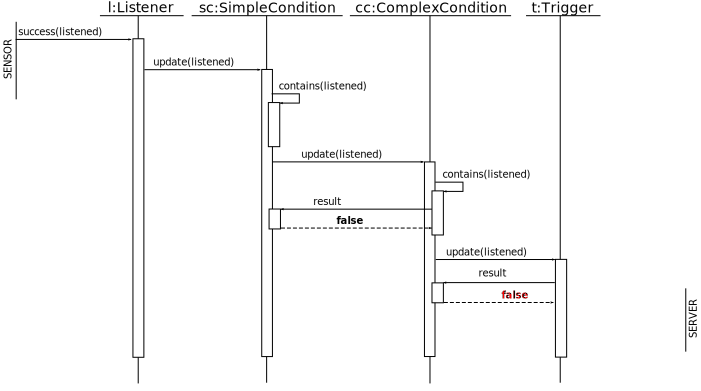
\includegraphics[scale=0.73]{SequenceNotificationFalseDiagram}
\caption{Diagrama de secuencia UML de la propagación hasta llegar al Trigger}
\label{SequenceNotificationFalseDiagram}
\end{figure}

El trigger es el que verifica si se debe notificar al servidor mediante la solicitud AJAX. Una forma de optmizar esto es frenar la propagación de la notificación en las condiciones previas, antes de que llegue al trigger, si es que la situación lo permite.

Para realizar esto se almacena el resultado de cada evaluación para cada condición. Esto permite verificar si la condición cambió de resultado con respecto a la evaluación anterior, permitiendo interrumpir la propagación en aquellos casos que lo requieran (ver Cuadro \ref{PropagationTable}).

\begin{table}[ht!]
\centering
\begin{tabular}{ | l | l l |}
\hline
anterior/actual & falso & verdadero \\
\hline
falso & para & continua \\
verdadero & continua & continua \\
\hline
\end{tabular}
\caption{Propagación de la notificación en las condiciones}
\label{PropagationTable}
\end{table}

Como se observa en la tabla cuando el resultado de la evaluación de una condición es \emph{falso}, y su resultado anterior fue \emph{falso} no es necesario notificar un cambio a los observadores de esta condición.


\section{Mecanismo de cancelación de una suscripción en el cliente}

Al considerar la interacción de un modelo con el contexto de sus usuarios, es posible contemplar que en algún momento el servidor deseará cancelar alguna de sus suscripciones.

Para poder realizar la cancelación es necesario que el servidor mantenga identificados todos los objetos enviados al cliente (triggers, condiciones simples y complejas). De esta forma puede especificarle al cliente cual de todos esos objetos quiere eliminar (o cancelar). Para lograrlo es necesario modificar la jerarquía de clases antes presentada, haciendo que la clase \emph{Condition} y la clase \emph{Trigger} extiendan a la clase \emph{ProxyObject} (ver Figura \ref{ProxyObjectHierarchy}).

\begin{figure}[ht!]
\centering
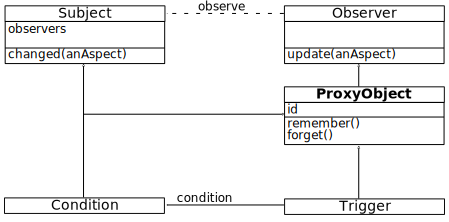
\includegraphics[scale=0.73]{ProxyObjectHierarchy}
\caption{Diagrama de clases UML con la clase ProxyObject}
\label{ProxyObjectHierarchy}
\end{figure}

Además la clase \emph{Contidion} continuará extendiendo a la clase \emph{Subject} para poder notificar a sus observadores en caso de ser necesario.

Por último es necesario subrayar que la clase \emph{ProxyObject} es la que permite reutilizar los \emph{sub-entornos} definidos utilizando instancias de la clase \emph{ComplexCondition}.


\section{Suscripción y desuscripción desde la perspectiva del servidor}

Teniendo en cuenta el esquema de notificaciones del cliente basados en el \emph{ProxyObject}, es necesario ampliar como el servidor construye la información para que luego pueda ser interpretada por el navegador web.

El proceso comienza cuando a una instancia de la clase \emph{Listener} (que reside en el servidor), asociada a un cliente en particular, se le envía el mensaje \emph{\#remember:} con una instancia de \emph{Trigger} como parámetro (ver Figura \ref{ServerSerializer}).

\begin{figure}[ht!]
\centering
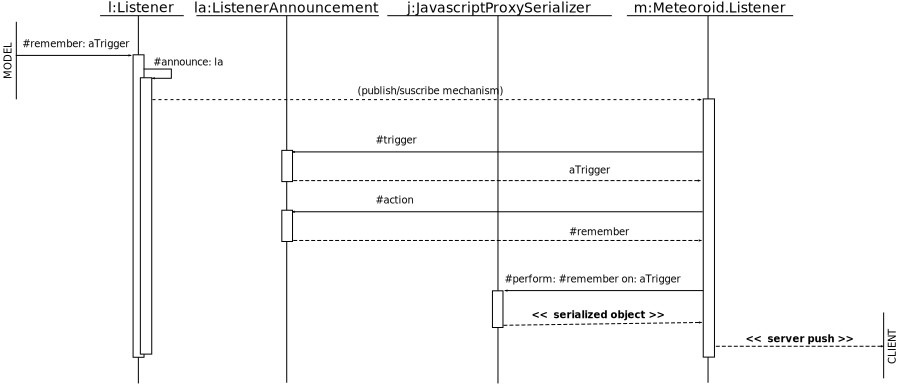
\includegraphics[scale=0.83,angle=90]{ServerSerializer}
\caption{Diagrama de secuencia UML de la serialización de objetos en el servidor}
\label{ServerSerializer}
\end{figure}

La instancia de la clase \emph{Listener} es observada por la clase \emph{Meteoroid.Listener}, que es un componente del framework \emph{Meteoroid}. Al utilizar el patrón de diseño \emph{Publish/Suscriber}, el componente de meteoroid es notificado cada vez que al Listener se le indica \emph{recordar} o \emph{olvidar} algún trigger.

Luego, al recibir una notificación la instancia de \emph{Meteoroid.Listener} le delega a una instancia de la clase \emph{JavascriptProxySerializer} para que recorra al objeto \emph{Trigger} con el fin de transformarlo en un código javascript adecuado para el navegador web.

El código javascript resultante describirá a las \emph{condiciones} que debe cumplir el entorno para ejecutar ese \emph{Trigger} y almacenará un \emph{callback de continuations} codificado como una solicitud de AJAX.

Por último, cuando el serializador devuelve el código javascript, el componente lo inyecta en el cliente (utilizando la técnica conocida como Server Push).


\section{Implementación de un sensor}

En las secciones anteriores se presentó el mecanismo de notificación de entornos en forma general. Este mecanismo le permite al servidor (basado en continuations) interactuar con un cliente dentro del dominio de la adaptabilidad al contexto. Para concluir con el entendimiento de lo explicado se prosigue con el desarrollo de un caso particular, como es el caso del \emph{sensor} de \emph{aceleración}.

Teniendo en cuenta que la aceleración proviene de un sensor altamente cambiante, el navegador web basado en \emph{Phonegap} provee en su API un método para configurar un \emph{timer}.

Para \emph{adaptar} esta API, se crea la clase \emph{AccelerationListener} (ver Figura \ref{AccelerationListenerClass}) que extiende a la clase \emph{Listener} e integra al sensor al mecanismo de notificaciones antes descripto.

\begin{figure}[ht!]
\begin{Verbatim}
AccelerationListener = Class.create(Listener, {
  initialize: function($super) {
    $super(1000);
  },
  sucess: function($super, listened) {
    _.listeners.acceleration.changed(listened);
    return true;
  },
  startListening: function() {
    this.timerId = navigator.accelerometer.watchAcceleration(
      this.sucess,
      this.fail,
      this.options
    );
  }
});

_.feel("acceleration", new AccelerationListener());
\end{Verbatim}
\caption{Código fuente de la clase AccelerationListener}
\label{AccelerationListenerClass}
\end{figure}

En el momento que este fragmento de código es interpretado por el navegador web, primero crea la clase \emph{AccelerationListener} y luego solicita al administrador de \emph{listeners} (clase \emph{ListenerManager}) para que agregue una instancia de la clase recién creada (linea 18). A partir de este momento una \emph{SimpleCondition} puede registrarse para escuchar una ``acceleration''.

En el proceso de creación de la instancia de la clase \emph{AccelerationListener}, por defecto se inicializa con una velocidad de refresco de \emph{1000 ms} que la clase \emph{Listener} se encargará de agregar al diccionario almacenado en el atributo \emph{options} (Ver linea 3 de la Figura \ref{AccelerationListenerClass}).

Luego, cuando se termine de cargar la página web, se le enviará un mensaje al método \emph{startListening} para que termine de configurar el \emph{timer} provisto por la interfaz de Phonegap (Ver linea 11 de la Figura \ref{AccelerationListenerClass}).

Cuando la aplicación web se encuentre corriendo en el cliente, cada vez que el \emph{timer} lo indique se llamará al método \emph{success}. Este último, se encarga de enviar el mensaje \emph{changed} a la instancia del listener para propagar la nueva lectura a todas las \emph{SimpleCondition} que lo estén observando (Ver linea 6 de la Figura \ref{AccelerationListenerClass}). A partir de esta propagación cada \emph{SimpleCondition} evaluará si contiene al valor propagado por el listener utilizando el atributo \emph{expression}.

Desde el punto de vista del desarrollador es necesario proporcionar una herramienta que simplifique la creación de condiciones. Para esto, en el servidor se implementa el patrón de diseño Builder explicado por \emph{Gamma et al.}\cite{Gamma95}.

Luego, para cada sensor se puede proporcionar un Builder que contemple los casos específicos de dicho sensor. Por ejemplo, para el caso del acelerómetro, se crea la clase \emph{OSCAccelerationBuilder} (ver Figura \ref{ServerBuilders}).

\begin{figure}[ht!]
\centering
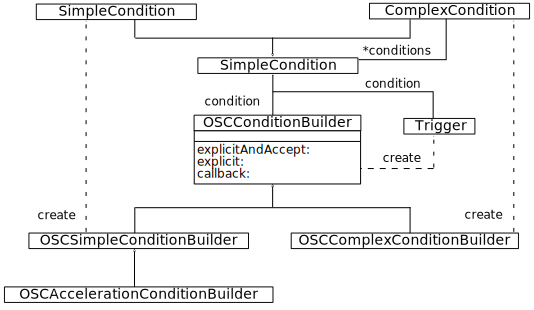
\includegraphics[scale=0.83]{ServerBuilders}
\caption{Diagrama de clases UML de la jerarquía de \emph{builders}}
\label{ServerBuilders}
\end{figure}

De esta forma, la clase \emph{OSCAccelerationBuilder} tiene la responsabilidad de construir instancias de la clase \emph{SimpleCondition} que serán atendidas por el listener que se encuentra del lado del cliente, registrado para atender condiciones de ``acceleration''.

Por último, como se observa en el diagrama de clases UML (Ver Figura \ref{ServerBuilders}) la librería cuenta con la clase \emph{OSCComplexConditionBuilder} que permite construir entornos complejos como consecuencia de agrupar un conjunto de condiciones.


\section{Visión global}

Con la misión de mantener, en la medida de lo posible, las características y propiedades de las aplicaciones web basadas en continuations, se diseña una extensión que permita la adaptación al contexto y mantienga la privacidad del usuario. Como se puede ver en el diagrama de clases \emph{UML}\footnote{Del inglés ``Unified Modeling Language''.} de la Figura \ref{UMLClassDiagram}, dicha extensión tiene dos partes, una se encuentra del lado del servidor y la otra del lado del cliente.

Para mantener dicha privacidad se plantea un esquema de notificaciones mediante el patrón de diseño \emph{Publish/Suscribe} que evita que el cliente deba enviar información detallada de los sensores al servidor. Para lograrlo, cada notificación del cliente solicitará al servidor que realice la ejecución de un \emph{callback de continuations} del framework \emph{Seaside}, de forma similar a la forma de procesar clicks en hipervinculos o botones.

\begin{figure}[ht!]
\centering
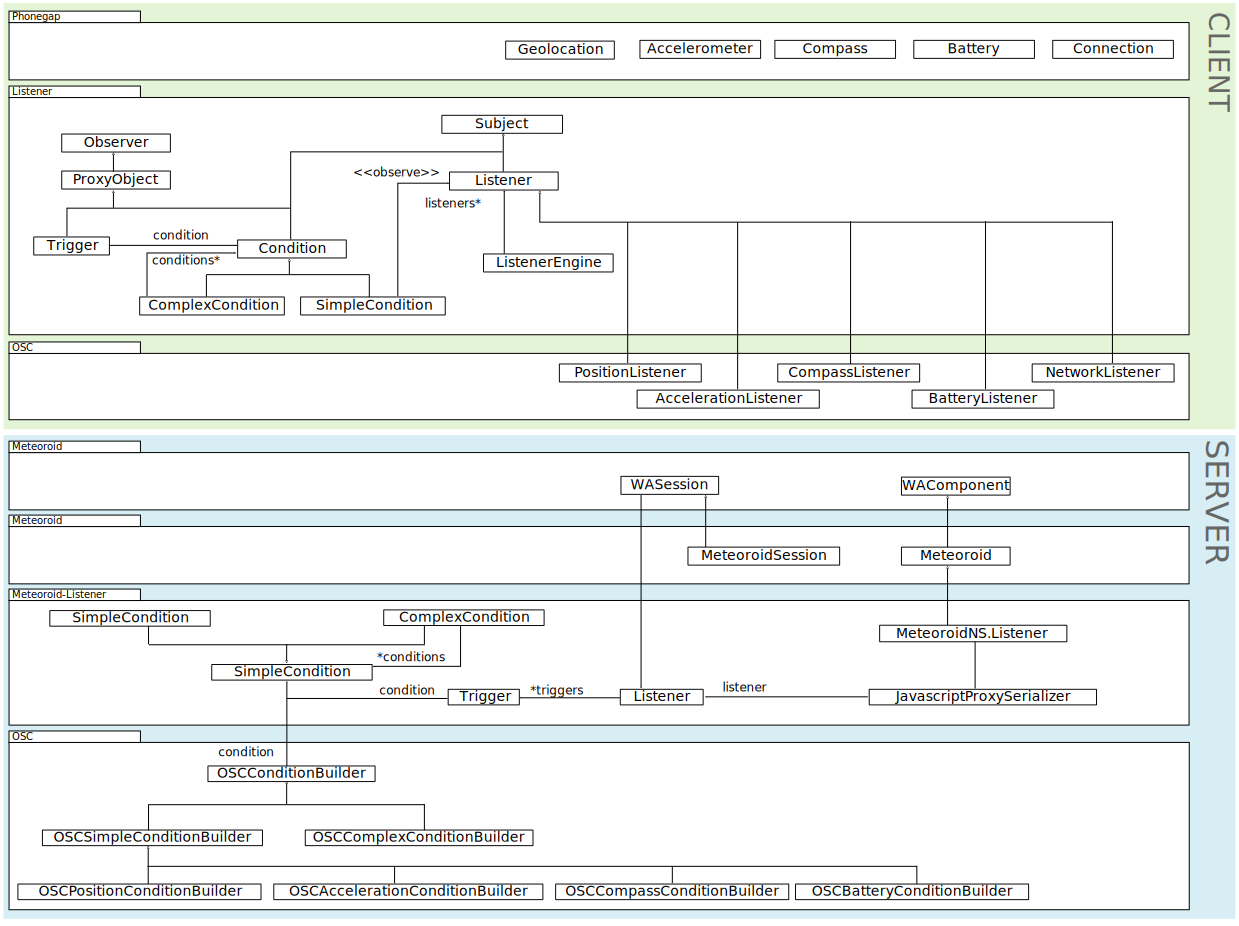
\includegraphics[scale=0.55,angle=90]{UMLClassDiagram}
\caption{Diagrama de clases UML de la extensión propuesta}
\label{UMLClassDiagram}
\end{figure}

% Chapter 5

\chapter{Caso de uso}
% Write in your own chapter title
\label{Capitulo 5}
\lhead{Capítulo 5. \emph{Caso de uso}} % Write in your own chapter title to set the page header

Con el objetivo de poner a prueba la librería presentada, en este capítulo se  describe como extender una aplicación web desarrollada con continuations para que pueda adaptarse al contexto.

Se utiliza como punto de partida una aplicación web que se encuentra en el repositorio publico de Cincom$ ^{\textregistered}$ dentro de los ejemplos de Seaside, e implementa una tienda \emph{on line} que permite encargar sushi.

Antes de agregar la sensibilidad al contexto, se reemplazan el tipo de producto por otro que pueda ser identificado con un código de barra. En este caso, se utilizarán libros.

Además, se le realizan modificaciones a los componentes de Seaside para utilizar Scriptaculous y Meteoroid con el fin de reducir la transferencia de datos y mejorar la velocidad de refresco de cada actualización\cite{Fernandez09}.

A continuación se detalla el modelo de negocio de la aplicación web previo a agregar la extensión. Luego se detallan los componentes de Seaside (junto con los de Scriptaculous y Meteoroid) que posibilitan la utilización del modelo. Para finalizar, una vez descripta la aplicación web, se explica como expandirla para proporcionar adaptabilidad al contexto.


\section{El modelo de negocio de la aplicación web}

El modelo de negocios de la tienda de libros consiste en registrar todas las ventas realizadas (clase Order). De cada venta se conoce el conjunto de libros que se solicitaron, la dirección de facturación y de entrega de los libros, y los datos de la tarjeta de crédito desde donde se realizó el pago (ver Figura \ref{WAStoreModel}).

\begin{figure}[ht!]
\centering
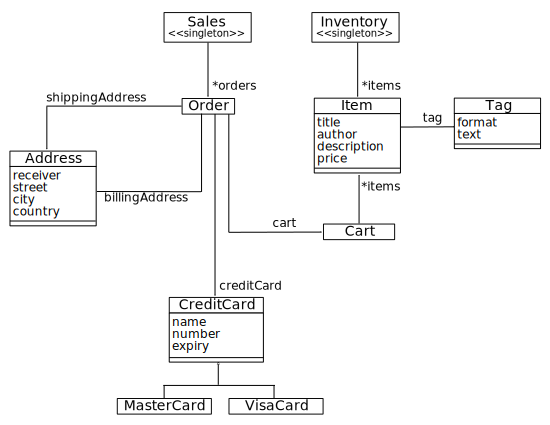
\includegraphics[scale=0.9]{UMLWAStoreModelClassDiagram}
\caption{Diagrama de clases UML del modelo de negocio de la tienda de libros}
\label{WAStoreModel}
\end{figure}

De cada libro (clase \emph{Item}) se conocen los atributos \emph{titulo}, \emph{autor/es}, \emph{descripción}, \emph{precio} y la \emph{descripción de un código de barras} (clase \emph{Tag}).

Las clases \emph{Sales} y \emph{Inventory} implementan el patrón de diseño \emph{Singleton}\cite{Gamma95}, y se encargan de almacenar las compras consumadas y los productos del inventario, respectivamente.


\section{La interfaz proporcionada por Seaside}

Para poder interactuar con el modelo existen un conjunto de componentes de Seaside, que dan forma a la aplicación web accesible por el usuario.

Mientras el usuario navega por la tienda on line, realiza consultas sobre el catálogo de productos (clase \emph{Inventory}, ver Figura \ref{bookstoreNetResultSequenceDiagram}). A su vez, puede agregar algún producto (clase \emph{Item}) a un carro de compras (clase \emph{Cart}), o sacarlo del carro de compras si es que ya no desea comprarlo (ver Figura \ref{bookstoreNetfillCartSequenceDiagram}).

\begin{figure}[ht!]
\centering
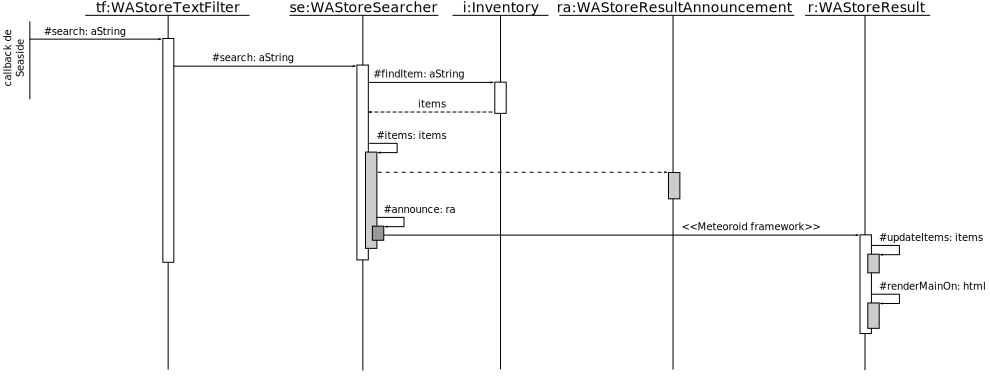
\includegraphics[scale=0.50]{bookstoreNetResultSeasideUMLSequenceDiagram}
\caption{Diagrama de secuencia UML de la búsqueda de productos}
\label{bookstoreNetResultSequenceDiagram}
\end{figure}

\begin{figure}[ht!]
\centering
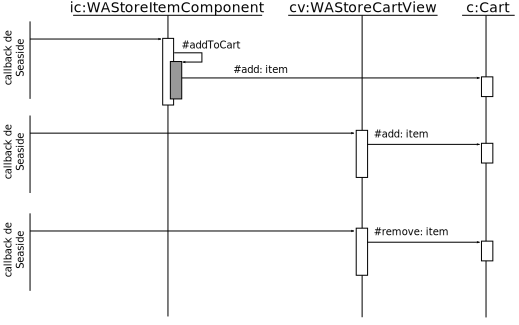
\includegraphics[scale=0.80]{bookstoreNetfillCartSeasideUMLSequenceDiagram}
\caption{Diagrama de secuencia UML de la carga de productos al carro de compras}
\label{bookstoreNetfillCartSequenceDiagram}
\end{figure}

Cuando el cliente desea hacer efectiva la compra, se le solicitan dos direcciones: una de envío del producto y otra para enviar la facturación (clase \emph{Address}). Para cada dirección deberá completar los atributos \emph{país}, \emph{ciudad}, \emph{calle} y \emph{nombre de la persona que recibirá} ya sea los libros o la facturación.

Por último, debe completar la información de su tarjeta de crédito (subclases de \emph{CreditCard}) y confirmar la compra. La confirmación de la compra significa la creación de una instancia de la clase \emph{Order} para registrar la compra. Esta instancia será automáticamente almacenada en la clase \emph{Sales} (ver Figura \ref{bookstoreNetSequenceDiagram}).

\begin{figure}[ht!]
\centering
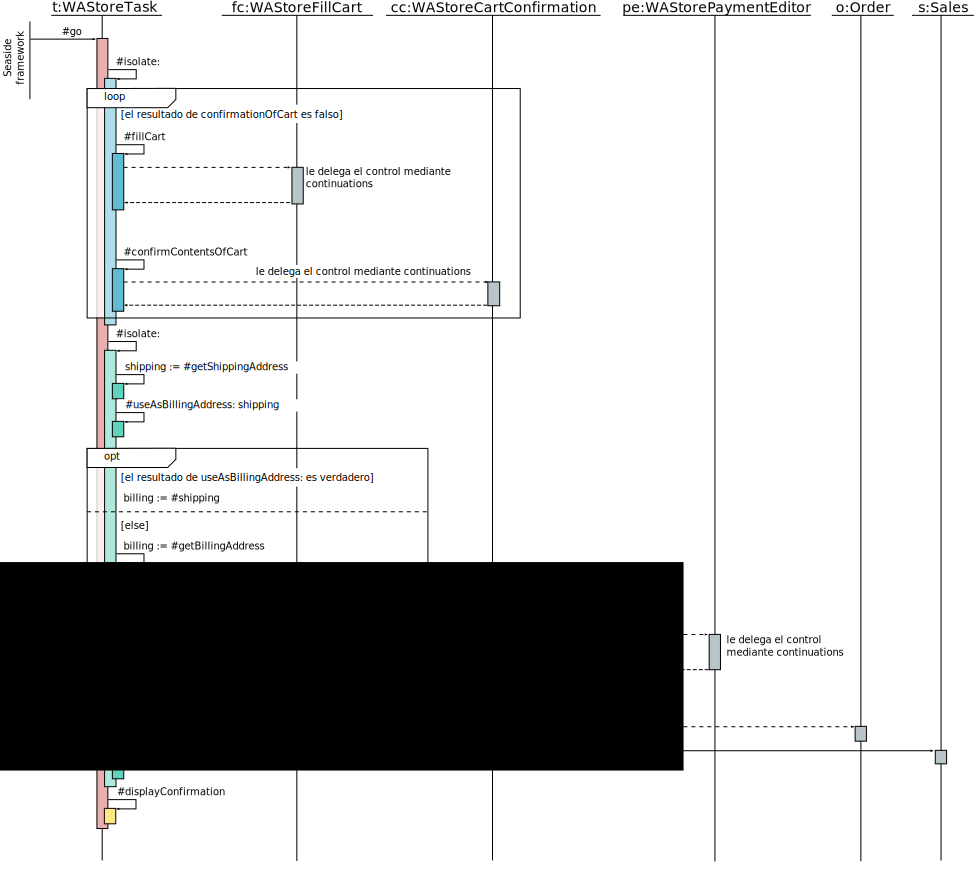
\includegraphics[scale=0.53]{bookstoreNetSeasideUMLSequenceDiagram}
\caption{Diagrama de secuencia UML de la tienda de libros}
\label{bookstoreNetSequenceDiagram}
\end{figure}

Es importante notar que en el método \emph{\#go} de la clase WAStoreTask se detalla el proceso completo, desde que el cliente se encuentra modificando el carro de compras, hasta que termina de abonar por la compra realizada. En esta descripción, se aíslan 2 subprocesos, la \emph{selección de los productos} y el \emph{pago}.

Una vez que se \emph{confirmó} la selección de los productos, el método \emph{\#isolate:} (perteneciente al framework Seaside) se encarga de descartar cualquier solicitud del navegador web que intente modificar el carro de compras. Lo mismo sucederá cuando se culmine de detallar la información de la tarjeta de crédito, bloqueando en este caso cualquier modificación de la orden generada.


\section{¿Cómo se utiliza la librería de adaptación al contexto?}

Si se extendiese el ejemplo presentado mencionando que la tienda de libros posee varios locales de venta al público en los que desea proveer un servicio adicional cuando un usuario (que se encuentra utilizando la aplicación web) accede. El servicio en cuestión, consiste en simplificar la búsqueda de la descripción y el precio de un articulo, a partir de la utilización de un código de barra.

El primer paso para proporcionar la sensibilidad al contexto es que el componente raíz de la aplicación web extienda a la clase \emph{MeteoroidNS.Meteoroid}.

Luego, es necesario agregar las librerías \emph{PhonegapLibrary}, \emph{ListenerEngineLibrary} y \emph{OSCLibrary} a la aplicación web. Por último se deberá agregar una variable de instancia para almacenar el componente \emph{MeteoroidNS.Listener}, que deberá ser \emph{renderizado} al final del método \emph{\#renderContentOn: html} del componente raíz.

A continuación para cumplir con los nuevos requisitos de la tienda de libros, se detallará el uso del sensor de posicionamiento para detectar que el usuario se encuentre dentro de un local de venta. Luego, se explicará el acelerómetro, el cual es necesario para detectar que el usuario desea escanear un código de barras. Y por ultimo, un \emph{sensor de códigos de barra} detectará si el código escaneado existe en el modelo de negocio.


\subsection{Sensor de posicionamiento}

Para detectar si el usuario se encuentra físicamente dentro de una tienda, es necesario establecer un polígono que delimite que posiciones pertenecen a una tienda. Luego, se utiliza a la librería para crear una \emph{Condition} que comprobará si la posición actual de un dispositivo se encuentra dentro de dicho polígono\footnote{Utilizando latitudes y longitudes como coordenadas.}. Por último, es necesario asociar esta condición a un \emph{trigger}, para que el servidor pueda coordinar la adaptación necesaria.

El código necesario para generar el trigger (ver Figura \ref{PositionInsideZoneExample}), primero crea a una instancia de la clase OSCPositionConditionBuilder al enviar el mensaje \emph{\#position} a la clase \emph{OSCConditionBuilder}.

\begin{figure}[ht!]
\begin{Verbatim}
insideTrigger := (OSCConditionBuilder position)
	inside: ((List new)
		add: -34.577301 @ -59.089359;
		add: -34.576801 @ -59.088829;
		add: -34.577690 @ -59.084999;
		add: -34.579041 @ -59.088242;
		add: -34.577793 @ -59.089119;
		add: -34.577339 @ -59.089279;
		add: -34.577301 @ -59.089359;
		yourself);
	callback: [self whenInside].
\end{Verbatim}
\caption{Código fuente para comprobar si una posición se encuentra en una zona}
\label{PositionInsideZoneExample}
\end{figure}

Como se desea conocer cuando el cliente ingresa a una tienda, se envía el método \emph{\#inside:} a la instancia del builder con una lista de posiciones como parámetro. Estas coordenadas determinan el perímetro de uno de los locales en particular (ver Figura \ref{satImageWithPolygon}).

\begin{figure}[ht!]
\centering
\includegraphics[scale=0.50]{satImageWithPolygon}
\caption{Mapa con el polígono en donde se encuentra la tienda}
\label{satImageWithPolygon}
\end{figure}

Luego, con el método \emph{\#callback:} se establece el comportamiento que debe realizar el servidor si el cliente \emph{dispara} ese \emph{trigger}. En este caso, enviará el mensaje \emph{\#whenInside} a la instancia que contenga la declaración anterior.

Dado que el trigger previo solo detecta cuando un usuario entra a una tienda, también es necesario controlar la condición opuesta para detectar cuando el cliente sale de la tienda, y en ese momento desactivar el servicio de búsquedas por código de barras

Lo único que será necesario cambiar será el método \emph{\#inside:} por \emph{\#outside:} (ver Figura \ref{PositionOutsideZoneExample}).

\begin{figure}[ht!]
\begin{Verbatim}
outsideTrigger := (OSCConditionBuilder position)
	outside: ((List new)
		add: -34.577301 @ -59.089359;
		add: -34.576801 @ -59.088829;
		add: -34.577690 @ -59.084999;
		add: -34.579041 @ -59.088242;
		add: -34.577793 @ -59.089119;
		add: -34.577339 @ -59.089279;
		add: -34.577301 @ -59.089359;
		yourself);
	callback: [self whenOutside].
\end{Verbatim}
\caption{Código fuente para comprobar si una posición se encuentra fuera de una zona}
\label{PositionOutsideZoneExample}
\end{figure}

A continuación, para que el servidor relacione a un trigger con un cliente en particular, es necesario solicitarle a una instancia de la clase \emph{Listener} (accesible desde la sesión de usuario de Seaside\footnote{Es importante destacar que todo el comportamiento de la sensibilidad al contexto se describe dentro de los \emph{WAComponent} de Seaside, y fuera del modelo de negocio.}) que lo \emph{recuerde} mediante el método \emph{\#remember:} (ver Figura \ref{PositionRememberListeningExample}).

\begin{figure}[ht!]
\begin{Verbatim}
self session listener remember: insideTrigger.
\end{Verbatim}
\caption{Código fuente para que un cliente sea sensible a un trigger.}
\label{PositionRememberListeningExample}
\end{figure}

Por el contrario, para que el navegador web deje de ser sensible a un \emph{trigger} deberá indicarle al \emph{listener} que lo \emph{olvide} utilizando el método \emph{\#forget:} (ver Figura \ref{PositionForgetListeningExample}).

\begin{figure}[ht!]
\begin{Verbatim}
self session listener forget: insideTrigger.
\end{Verbatim}
\caption{Código fuente para que un cliente deje de ser sensible a un trigger.}
\label{PositionForgetListeningExample}
\end{figure}

\subsection{Sensor de aceleración}

Luego de detectar la posición del usuario, si este se encuentra en una tienda es necesario reconocer si su intención es escanear un código de barras.

Para lograr esto, cuando se encuentra dentro de una tienda (el método \emph{\#whenInside}), se deberán registrar que posturas del dispositivo activarán la lectura de códigos de barra y en que posturas estas deberían desactivarse.

Por ejemplo, cuando el dispositivo se encuentra de forma vertical se asume que el usuario se encuentra en una postura ideal para utilizar la aplicación web. Por el contrario, cuando el usuario posiciona el dispositivo en forma apaisada, será interpretado como que el usuario desea leer un código de barras (ver Figura \ref{devicePostures}).

\begin{figure}[ht!]
\centering
\includegraphics[scale=0.50]{devicePostures}
\caption{Postura vertical y horizontal de un dispositivo}
\label{devicePostures}
\end{figure}

Al describir la postura de escaneo de códigos de barra se tiene en cuenta cierta movilidad o margen de error mostrado en la \emph{vista lateral}. Esta flexibilidad permitirá rotar hacia atrás el dispositivo cuando se encuentra en horizontal.

Luego, para definir la postura de escaneo es necesario utilizar 2 triggers, uno para cada tipo de apaisamiento. El primer trigger se encargará de detectar un angulo de 90 grados desde la posición vertical en sentido contrario a las agujas del reloj, mientras que segundo trigger se encargará de los 90 grados en sentido horario.

Teniendo en cuenta los extremos para cada una de las posturas se plantea como valores medios los puntos [x:7, y:0, z:5] y [x:-7, y:0, z:5] (ver Figura \ref{ScanBarcodePostureExample}). Luego el margen de error es para ambas posturas iguales [x:5, y:1, z:5]\footnote{Al eje del acelrómetro \emph{y} se le deja un margen de error de $\pm1$ $m/s^2$ para que el usuario pueda encontrar de forma sencilla la postura para escanear el código de barra, y no tenga que lidiar con la sensibilidad ofrecida por los acelerómetros de distintos dispositivos.}

\begin{figure}[ht!]
\begin{Verbatim}
scanningPosture1 := (OSCConditionBuilder acceleration)
	when: 7 @ (0 @ 5);
	acceptError: 5 @ (1 @ 5);
	callback: [self wantScanBarcodes].
scanningPosture2 := (OSCConditionBuilder acceleration)
	when: -7 @ (0 @ 5);
	acceptError: 5 @ (1 @ 5);
	callback: [self wantScanBarcodes].
\end{Verbatim}
\caption{Código fuente para describir la postura de escaneo de código de barras}
\label{ScanBarcodePostureExample}
\end{figure}

Nuevamente, es necesario recordar que habrá que informarle al \emph{Listener} de la sesión del usuario mediante el método \emph{\#remember:} si es que deseamos reconocer este entorno.

Por otra parte, se determina que el usuario quiere navegar por la aplicación web cuando no se encuentra en una postura de escaneo. Para identificar esto se define un trigger con una condición compleja (ver Figura \ref{NavigationPostureExample}).

\begin{figure}[ht!]
\begin{Verbatim}
navigationPosture := (OSCConditionBuilder complex)
	when: [:env |
		((env acceleration)
			whenNot: -7 @ (0 @ 5);
			acceptError: 5 @ (1 @ 5))
		&
		((env acceleration)
			whenNot: 7 @ (0 @ 5);
			acceptError: 5 @ (1 @ 5))];
	callback: [self wantNavigate].
\end{Verbatim}
\caption{Código fuente para describir la postura de escaneo de código de barras}
\label{NavigationPostureExample}
\end{figure}

Dentro del bloque de código que se le pasa como parámetro al método \emph{\#when:}, la variable \emph{env} permitirá acceder a la clase \emph{OSCConditionBuilder} dentro de la condición compleja. También es importante notar el método \emph{\#whenNot:} que niega la ocurrencia de esa condición. Por último, el operador \& (comúnmente llamado ``and'') permite la concatenación de condiciones para formar una más compleja.


\subsection{Sensor de códigos de barra}

En el momento que el \emph{acelerómetro} detecte que el usuario se encuentra en la postura adecuada para escanear un código de barra, la aplicación web deberá cargar en el dispositivo móvil del cliente los triggers adecuados para reconocer el código de barra de cada libro (ver Figura \ref{BarcodeTriggerExample}).

\begin{figure}[ht!]
\begin{Verbatim}
bookTriggers := OrderedCollection new.
Inventory default allItems do: [:item | 
	bookTriggers add: ((OSCConditionBuilder tag)
		when: item tag format | item tag text;
		callback: [ self findTaggedWith: item tag ])]
\end{Verbatim}
\caption{Código fuente para describir las condiciones relacionadas con códigos de barras aceptados por el modelo}
\label{BarcodeTriggerExample}
\end{figure}

En este caso se agregan todos los triggers a una colección de objetos, notar que en el método \emph{\#when:} se envía como parámetro el \emph{formato} del código y el \emph{texto} que simboliza la secuencia de caracteres o dígitos del código.

Para finalizar será necesario solicitarle al \emph{Listener} de la sesión del usuario que recuerde cada uno de los triggers contenidos en la colección \emph{bookTriggers}, para que el navegador pueda utilizarlos para reconocer entornos\footnote{Del lado del cliente, el navegador solo mostrará la pantalla de escaneo de códigos de barras si es que existe alguna condición dentro del \emph{listener} de códigos de barras.}.

Como consecuencia del proceso anterior, si el cliente enfoca la cámara de su dispositivo hacia el código de barras de un libro, el navegador web procederá a mostrar la información relacionada con dicho libro.

Cabe señalar que así como se describieron estos sensores, necesarios para desarrollar el caso de uso planteado, existen otros (como el estado de la batería, el tipo de conexión a internet, la orientación con respecto al Polo Norte, etc.) que también pueden ser utilizados. Además, si la situación lo requiere, se pueden crear una gran cantidad de nuevos sensores que ayuden a reconocer las necesidades del usuario.

% Chapter 6

\chapter{Extensibilidad y límites}
% Write in your own chapter title
\label{Capitulo 6}
\lhead{Capitulo 6. \emph{Extensibilidad y límites}} % Write in your own chapter title to set the page header

Como consecuencia de la librería presentada se desprenden posibles desarrollos y extensiones que podrían mejorar la adaptabilidad al contexto, o por otra parte, la privacidad y la seguridad del usuario.

Por otra parte, dado que al realizar la librería se han tomado ciertas decisiones de diseño, habrá limites que no podrán ser solucionados mediante las extensiones. Por esto, es necesario describir cuales serán los límites de la librería con motivo de determinar el alcance de la solución planteada.

A continuación se presentan algunas de las extensiones posibles relacionadas con las distintas lineas de investigación en las que se sostiene esta tesis. Por último se prosigue con la descripción de los limites encontrados y se mencionan que características de la sensibilidad al contexto no podrán utilizarse si se mantiene lo propuesto en esta tesis.


\section{Extensibilidad}

Al momento de desarrollar la librería surgieron diferentes ideas que son las que le dieron forma, pero también existieron otras opciones que fueron pospuestas en pos de acotar el alcance de la tesis.

Estas posibles extensiones pueden ser clasificadas en: las que agregan nuevos \emph{sensores} al navegador web mediante \emph{plugins}; y las que mejoran la privacidad y seguridad del usuario.

En el primer grupo, se encuentran aquellos nuevos sensores que permitirán reconocer de forma mas precisa el contexto. Estos sensores podrán reconocer distintas características del contexto como la temperatura, la humedad, la presión atmosférica, u otros entornos aún no pensados.

Dentro de este mismo grupo, también se pueden crear sensores que notifiquen a cada aplicación web los recursos con los que cuenta para realizar su ejecución, y así proporcionarle mayor información sobre las capacidades que el dispositivo está dispuesto a proporcionarle en un momento particular. Por ejemplo, notificarle cuando se le brinda mas capacidad de procesamiento o cuando se le quita dicho recurso.

Dicha información permitirá establecer requisitos mínimos sobre ciertos recursos del dispositivo móvil, permitiendo descartar ciertas adaptaciones si es que el dispositivo no es capaz de procesarlas de forma adecuada.

A su vez, al profundizar este último caso, es necesario contemplar la ejecución en paralelo de distintas aplicaciones web e identificar la necesidad de un método que permita su \emph{interacción} (semejante a lo planteado por \emph{Efstratiou}\cite[p.~5]{Efstratiou04}).

En el segundo grupo, se encuentran aquellas ideas que modifiquen la administración de privacidad relacionada con los sensores, mediante una mayor flexibilidad de la interfaz gráfica o a través de la simplificación la interacción con el usuario.

Existen varias alternativas de investigación dentro de este grupo. Primero, sería interesante evaluar si la utilización del patrón de diseño \emph{Composite}\cite[p.~151]{Gamma95} mejora la interfaz de administración de permisos. Luego, queda pendiente verificar si la utilización de \emph{permisos asociativos}\footnote{El \emph{permiso asociativo} consiste en definir el permiso de una aplicación A a partir de los permisos concedidos a otras aplicaciones B y C.} simplifica la administración de accesos o solo le quita transparencia al proceso. Por último, quedaría corroborar como afectan estas nuevas estrategias de permisos y accesos al \emph{Same Origin Policy (SOP)}\footnote{
La \emph{Same Origin Policy} es una regla que establece que un \emph{script} de Javascript solo se pueda acceder a los métodos y propiedades asociados a su origen, restringiendo el intercambio de información entre scripts de distintos orígenes.} presente en los navegadores web.

Dentro de ésta segunda agrupación, cada modificación puede ser evaluada teniendo en cuenta la usabilidad que le proporciona al usuario y la maleabilidad para establecer permisos entre las distintas aplicaciones web.


\subsection{Interacción entre aplicaciones web}

En el uso cotidiano de un navegador web es habitual la carga y ejecución en simultaneo de varias aplicaciones web, aunque se visualice solo una de ellas. Estas ejecuciones concurrentes de aplicaciones, combinadas de forma inadecuada con la adaptación al contexto, puede producir los inconvenientes ya planteados por \emph{Efstratiou}\cite[p.~5]{Efstratiou04}.

En particular, \emph{Efstratiou} presenta un escenario en donde existen una aplicación sensible al consumo energético y otra que es sensible al ancho de banda de una red inalámbrica (por ejemplo un reproductor de música de una radio online).

En un punto de la ejecución, la primer aplicación reduce el consumo de ancho de banda de la red con el fin de reducir el consumo energético. Al instante sucesivo, la segunda aplicación encuentra que puede aumentar la calidad del audio dado que el sistema dispone de un mayor ancho de banda recientemente libreado por la primer aplicación.

Como resultado de estas adaptaciones independientes, las acciones de adaptación de la primera aplicación serán canceladas por las adaptaciones realizadas de la segunda. Para sobrellevar esto \emph{Efstratiou} plantea una solución en conjunto en donde se contemplan los requisitos y las prioridades de cada aplicación \cite[p.~58]{Efstratiou04}. En esta linea queda pendiente analizar la solución teniendo en cuenta la utilización de continuations y los requisitos de seguridad existentes en los navegadores web.

Esta última linea, a su vez, se puede continuar mediante el análisis de la capacidad de intercomunicar dos aplicaciones web mediante un canal proporcionado por el navegador web.

Un canal de tales características podría mejorar el rendimiento de ambas aplicaciones al proveer un mecanismo de sincronización, este mecanismo podría permitir la colaboración entre las distintas aplicaciones web y por consecuencia evitar el procesamiento por duplicado.

En este tipo de comunicación entre aplicaciones, también debería contemplarse algún tipo de control para mantener la seguridad de la aplicación.


\subsubsection{Administración de permisos mediante Composite}

Teniendo en cuenta que el diseño presentado promociona la creación de una gran cantidad de sensores, en un futuro surgirá la necesidad de mejorar la administración de accesos para que un usuario sea capaz de discernir y decidir que información desea compartir con cada una de las aplicaciones web.

El módulo de administración tendrá que considerar que cada aplicación web puede requerir una configuración distinta de accesos, y deberá evaluar cada cuando tiempo un usuario modifica los permisos ya concedidos para una aplicación web particular.

El patrón de diseño Composite puede ser una estructura válida para proveer una gran granularidad en el control de los permisos y aún así, en caso de necesidad, permitir la abstracción mediante la agrupación de alguno de estos permisos; ya sean estos simples o consecuencia de otra agrupación previa.

En este planteo se deberá investigar si existen grupos de permisos que se repiten en diferentes aplicaciones. Y, por otra parte, si la agrupación en si misma simplifica la tarea de configuración de permisos que suele llevar a cabo el usuario.


\subsubsection{Permisos asociativos}

Ya sea como complemento del caso anterior, o como investigación individual, puede llegar a tener cierta connotación la posibilidad de determinar los permisos de una aplicación web a partir de la unión de permisos de una o mas aplicaciones web.

En este tipo de estrategia de administración el foco se centra en establecer los permisos a partir de semejanzas con otras aplicaciones web. Dada una aplicación web que fue desarrollada por una organización, una segunda aplicación web de esta organización recibiría como mínimo los mismos permisos que la primera aplicación desarrollada.

Y, mediante este enfoque, el usuario podría establecer explícitamente desde una interfaz gráfica que los permisos de la segunda aplicación web son idénticos a los de la primera. De esta forma, si los permisos concedidos a la primera se modificasen, la segunda aplicación web automáticamente conocería las mismas restricciones.

En esta linea se deberá analizar si el usuario es capaz de discernir en todo momento los permisos que se encuentra administrando.


\subsubsection{Estrategias para extender el Same Origin Policy}

Aunque en el ejemplo considerado en el capítulo \ref{Capitulo 5} toda la aplicación se descarga desde el mismo \emph{origen}\footnote{Un \emph{orígen} se encuentra definido por el \emph{dominio}, \emph{puerto} y el \emph{protocolo} utilizados en una \emph{URL} particular.}, es posible que en otros casos la aplicación web se descargue desde múltiples \emph{orígenes}. Teniendo en cuenta dicha situación, es necesario evaluar una solución que permita conceder distintos niveles de permisos para cada origen.

Dos posibles soluciones a este problema podrían ser: permitir solo al origen principal acceder a la información de los sensores, o distinguir orígenes secundarios y permitir una administración de permisos mas detallada.

En la primer solución, será necesario realizar la extensión correspondiente a la Same Origin Policy bloqueando cualquier tipo de acceso a los orígenes secundarios.

Por otra parte, para la segunda solución, deberán considerarse alternativas mas dinámicas de administración de permisos que simplifiquen y clarifiquen las selecciones realizadas por el usuario en cuanto a la información que desea compartir. En este punto volverían a tener vigencia tanto los \emph{permisos asociativos}, como los \emph{permisos mediante Composite}.


\section{Limites}

Al considerar la flexibilidad proporcionada por la creación de nuevos sensores, también es necesario analizar cuales serán los limites de este diseño.

La base del diseño consiste en que la aplicación web proporcione una mayor privacidad al usuario al utilizar \emph{triggers} y notificar al servidor solo en caso de que un \emph{entorno} se cumpla.

Al proteger la información de los sensores manteniéndola del lado del cliente y solo notificar lo indispensable al servidor, este último nunca recibirá información como para realizar un análisis complejo que le permita detectar nuevos patrones de comportamiento del cliente.

Esta situación es la que determina que el servidor nunca podrá implementar la característica evolutiva de la sensibilidad al contexto.


% Chapter 7

\chapter{Conclusión}
% Write in your own chapter title
\label{Capitulo 7}
\lhead{Capitulo 7. \emph{Conclusión}} % Write in your own chapter title to set the page header

Como consecuencia del diseño y el desarrollo realizados, ha quedado demostrada la existencia de una alternativa que permita a una aplicación web desarrollada con continuations utilizar los sensores de un dispositivo.

Teniendo en cuenta los objetivos de esta tesis y las características de las posibles extensiones, y habiendo contemplando a su vez los límites de la idea presentada, a continuación se realizará una comparación con otros trabajos de semejantes características.

Luego se enumerarán los resultados obtenidos a partir del diseño propuesto. Y por último se presentarán algunos de las trabajos pendientes que requieren de un análisis mas profundo.


\section{Trabajos relacionados}
\label{Trabajos Relacionados}

En la introducción a este documento se mencionaron otros trabajos que mantienen relación con alguna de las lineas de investigación desarrolladas. Para distinguir el aporte realizado por este trabajo se procede con la descripción de las principales diferencias entre el diseño presentado y el enfoque presentado por el resto de los trabajos.

Al contemplar el aporte realizado por \emph{Queinnec}\cite{Queinnec01}, que resuelve los inconvenientes relacionados con las transacciones y los estados de una aplicación web mediante la utilización de Continuations, este diseño no hace mas que agregar una extensión que permita el manejo de información contextual a este tipo de aplicaciones.

Luego, siguiendo por la linea de las aplicaciones web se encuentra el trabajo de \emph{Challiol et al.}\cite{Challiol06}, que ha sido desarrollado con MVC. En este trabajo se implementa un Controlador que es el encargado de manejar la información contextual, aunque esta solo consista en información de localización, que puede ser obtenida por múltiples sensores que se encuentran distribuidos en el ambiente.

A diferencia de \emph{Challiol et al.}, en este trabajo se presentan ejemplos en los que se restringe la ubicuidad de los sensores y se determina que la información es siempre proporcionada por el dispositivo móvil del cliente, con el fin que el usuario siempre tenga el control de su privacidad. Además los valores leídos por los sensores nunca son enviados a los servidores, con el fin de mejorar la privacidad y seguridad del usuario.

Por otra parte \emph{Chang et al.}\cite{Chang07} plantea un mecanismo de adaptación web que se enfoca en incorporar la sensibilidad al contexto contemplando principalmente la QoS. Su enfoque consiste en decidir de que lado de la conexión conviene ejecutar una serie de bloques (o componentes). Este tipo de adaptación puede ser realizada solo en el momento que la aplicación web se carga en el cliente, perdiendo la aplicación cualquier posibilidad de realizar nuevas adaptaciones en tiempo de ejecución.

A diferencia de \emph{Chang et al.}, en este trabajo se provee mayor flexibilidad para decidir el momento de aplicar una adaptación. Por otro lado, \emph{Chang et al.} contempla la variante evolutiva al momento de diseñar su modelo.

En el 2009, \emph{Kapitsaki et al.}\cite{Kapitsaki09} define que una forma de permitir la sensibilidad al contexto es mediante la composición de un servicio o aplicación web con un servicio de sensibilidad al contexto, mediante la utilización de otro servicio web que se encarga de la composición. Esto implica que la sensibilidad al contexto queda definida fuera del modelo de negocios.

Parte de estas nociones, proporcionadas por \emph{Kapitsaki et al.}, han sido utilizadas al momento de definir como se relaciona la sensibilidad al contexto con el modelo de negocio. A diferencia de \emph{Kapitsaki et al.}, en este trabajo, la composición entre la sensibilidad al contexto y el modelo de negocio ocurren dentro de los componentes de Seaside.

El resto de los trabajos (\emph{Efstratiou}\cite{Efstratiou04} y \emph{Fortier et al.}\cite{Fortier09}) se encuentran relacionados con la sensibilidad al contexto y proponen el desarrollo de aplicaciones que no corren en navegadores web, por lo que la privacidad del usuario nunca surgió como un tópico a analizar.

El trabajo de \emph{Efstratiou}\cite{Efstratiou04} consiste en desarrollar un procedimiento basado en pólizas que permite administrar de forma coordinada las adaptaciones sugeridas por múltiples aplicaciones. Estas pólizas consisten en disparar \emph{triggers} para llevar a cabo las adaptaciones necesarias.

Aunque en el diseño presentado en el capítulo \ref{Capitulo 4} se utiliza el concepto de triggers de \emph{Efstratiou} y se mencionan posibles extensiones que produzcan una adaptación coordinada, fue necesario adaptar lo propuesto por \emph{Efstratiou} a una arquitectura de aplicaciones web basada en Continuations.

En comparación con la propuesta de \emph{Costanza}\cite{Costanza08}, que presenta el \emph{COP} como un nuevo paradigma, esta librería tiene un alcance mas limitado que es brindar sensibilidad al contexto a aplicaciones web desarrolladas con continuations.

Por último \emph{Fortier et al.}\cite{Fortier09}, plantea una plataforma para tratar con la complejidad de un software sensible al contexto. Esta plataforma está compuesta por 4 partes: el \emph{soporte de sensibilidad}, las \emph{adaptaciones específicas del dominio}, un \emph{adaptador a aplicaciones existentes} y por último el módulo de conexión de las tres partes anteriores compuesto por \emph{abstracciones centrales}.

La principal diferencia con el diseño de \emph{Fortier et al.} consiste en el punto de conexión entre el modelo contextual y el modelo de negocio. \emph{Fortier et al.} considera que el modelo contextual se encuentra directamente relacionado con el modelo de negocios, de esta forma se torna mas difícil que cada interfaz de usuario establezca nuevas formas de comunicar ambos modelos (el contextual y el de negocios).

Para sobrellevar dicha situación, en este documento se presentó un lenguaje que permite definir la relación entre el modelo contextual y el modelo de negocios dentro de una subclase de Component (que se utilizan para definir interfaces en Seaside).


\section{Lecciones aprendidas}

Al concluir este trabajo se ha logrado cumplir con tres los objetivos que lo motivaron: El desarrollo, la explicación mediante patrónes de diseño y la comparación con otras alternativas. 

En primer lugar, se ha proporcionado un mecanismo para que una aplicación web desarrollada con continuations se pueda adaptar al contexto del usuario. Esta adaptación permitirá que aplicaciones web que en la actualidad se encuentran realizadas con continuations puedan a su vez adaptarse al contexto.

Luego, se han explicado las decisiones de diseño mediante la utilización de patrónes de diseño como: \emph{Adapter}, \emph{Composite}, \emph{Publish/Subscriber} y \emph{Builder}.

El \emph{Adapter} ha permitido estandarizar las interfaces de los posibles sensores para que la utilización de sus valores pueda realizarse mediante condiciones preestablecidas.

Luego, el \emph{Composite} ha proporcionado flexibilidad y simplicidad para combinar distintas condiciones, permitiendo a su vez realizar ciertas optimizaciones en el procesamiento.

Posteriormente, el \emph{Publish/Subscriber} ha otorgado una forma de mantener la privacidad del usuario, además de reducir el uso de la red en comparación con otras alternativas basadas en MVC.

El \emph{Builder}, por otra parte, ha simplificado la forma de definir condiciones, permitiendo que el desarrollador siga enfocado el la lógica del negocio, y ahora con la posibilidad de aprovechar la información contextual.

Por último, en la sección \nameref{Trabajos Relacionados} (\ref{Trabajos Relacionados}) se ha realizado una breve mención de las diferencias existentes con otras alternativas.


\section{Trabajo futuro}

Luego de la conclusión del objetivo planteado en este documento, y considerando las distintas alternativas para continuar esta nueva linea de investigación\footnote{Considerando que es necesaria una linea de investigación que se enfoque en analizar a las aplicaciones web basadas en continuations en combinación con la sensibilidad al contexto.}, en un futuro me encontraré analizando el rendimiento, en términos de necesidad computacional y de comunicación de la sensibilidad al contexto, entre las aplicaciones web basadas en continuations y aquellas que utilizan el esquema MVC.

En esta linea, también ha quedado pendiente mejorar los Builders de condiciones tanto simples como complejas de forma tal que utilicen todas las posibilidades de la \emph{lógica difusa} para definir los diferentes entornos.

Por otra parte, dentro del navegador web, es necesario analizar la definición de una API que estandarice la definición de sensores. De esta forma reducirá la necesidad de definir el comportamiento específico de cada \emph{Listener} del lado de \emph{javascript}.

Además, analizaré que posibilidades hay de definir una Ontología que permita la utilización de nuevos sensores sin la necesidad de modificación del navegador web. Esto permitirá agregar nuevos sensores, sin la necesidad de volver a compilar el navegador web. En esta linea, tal vez sea posible detectar de forma automática que sensores se encuentran disponibles en un dispositivo, y ponerlos a disposición para que el usuario pueda utilizarlos.

En otro aspecto, es necesario mejorar e investigar una alternativa que mejore la percepción del usuario en torno a la administración del acceso y la información privada. En esta etapa, será necesario realizar un análisis de usabilidad de la interfaz de configuración y ofrecer una alternativa que sea simple e intuitiva.

Por último, continuando con la administración del acceso, también me enfocaré en analizar la \emph{interacción entre aplicaciones web}, la \emph{administración de permisos mediante Composite}, los \emph{permisos asociativos} y 	posibles \emph{estrategias para extender el Same Origin Policy} (Ver el capítulo \ref{Capitulo 6}, \nameref{Capitulo 6}).

%% ----------------------------------------------------------------
% Now begin the Appendices, including them as separate files

%\addtocontents{toc}{\vspace{2em}} % Add a gap in the Contents, for aesthetics

%\appendix % Cue to tell LaTeX that the following 'chapters' are Appendices

\addtocontents{toc}{\vspace{2em}}  % Add a gap in the Contents, for aesthetics
\backmatter

%% ----------------------------------------------------------------
\label{Bibliography}
\lhead{\emph{Referencias bibliográficas}}  % Change the left side page header to "Bibliography"
\bibliographystyle{unsrtnat}  % Use the "unsrtnat" BibTeX style for formatting the Bibliography
\bibliography{References/Bibliography}  % The references (bibliography) information are stored in the file named "Bibliography.bib"

\begin{empcmds}
end
\end{empcmds}
\end{empfile}
\end{document}  % The End
%% ----------------------------------------------------------------
